%%%%%%%%%%%%%%%%%%%%%%%%%%%%%%%%%%%%%%%%%%%%%%%%%%%
\begin{frame}
  \begin{center}
    {\Large Convolutional Neural Network (CNN)}
  \end{center}
\end{frame}

%%%%%%%%%%%%%%%%%%%%%%%%%%%%%%%%%%%%%%%%%%%%%%%%%%%
\begin{frame}
  \begin{center}
    {\Large Introduction}
  \end{center}
\end{frame}

%%%%%%%%%%%%%%%%%%%%%%%%%%%%%%%%%%%%%%%%%%%%%%%%%%%
\begin{frame}[fragile] \frametitle{Images}

\begin{center}
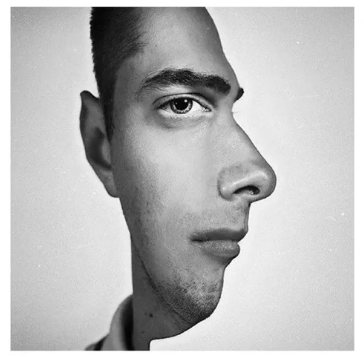
\includegraphics[width=0.4\linewidth,keepaspectratio]{cnn38}

\tiny{(Ref: Deep Learning A-Z - Kirill Eremenko)}
\end{center}

\begin{itemize}
\item  Do you see a person looking at you or to the right?
\item Brain struggles.
\item if you look at right edge, something. If left, something else.
\item Brain is trying to detect based on Features.
\end{itemize}


\end{frame}

%%%%%%%%%%%%%%%%%%%%%%%%%%%%%%%%%%%%%%%%%%%%%%%%%%%
\begin{frame}[fragile] \frametitle{Images}

\begin{center}
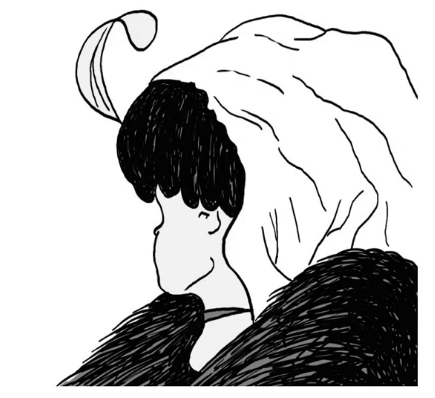
\includegraphics[width=0.35\linewidth,keepaspectratio]{cnn39}

\tiny{(Ref: Deep Learning A-Z - Kirill Eremenko)}
\end{center}

\begin{itemize}
\item Is it a young girl looking away or an old lady looking downwards.
\item Just one or two features are not sufficient at times, need more clues ie more differentiable features.
\end{itemize}

\end{frame}

%%%%%%%%%%%%%%%%%%%%%%%%%%%%%%%%%%%%%%%%%%%%%%%%%%%
\begin{frame}[fragile] \frametitle{Images}

\begin{center}
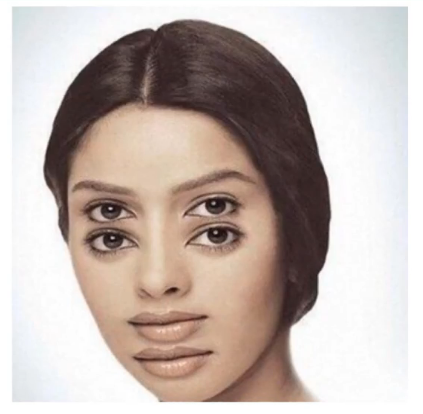
\includegraphics[width=0.4\linewidth,keepaspectratio]{cnn40}

\tiny{(Ref: Deep Learning A-Z - Kirill Eremenko)}
\end{center}

\begin{itemize}
\item Brain can not detect at times.
\item We sometimes get confused, Eisher's diagrams, anyone?
\end{itemize}


\end{frame}

%%%%%%%%%%%%%%%%%%%%%%%%%%%%%%%%%%%%%%%%%%%%%%%%%%%
\begin{frame}[fragile] \frametitle{Images}

\begin{center}
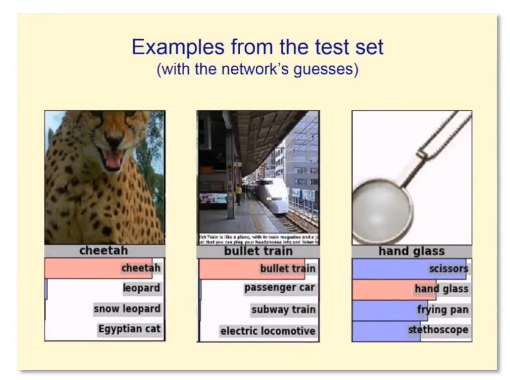
\includegraphics[width=0.5\linewidth,keepaspectratio]{cnn41}

\tiny{(Ref: Deep Learning A-Z - Kirill Eremenko)}
\end{center}

\begin{itemize}
\item Geoffrey Hinton, Yann Lecun are the pioneers of Image related Neural Networks, Convolution Neural Networks (CNN)
\item Their results were promising but confusing at times.
\end{itemize}


\end{frame}

%%%%%%%%%%%%%%%%%%%%%%%%%%%%%%%%%%%%%%%%%%%%%%%%%%%
\begin{frame}
  \begin{center}
    {\Large CNN}
  \end{center}
\end{frame}

%%%%%%%%%%%%%%%%%%%%%%%%%%%%%%%%%%%%%%%%%%%%%%%%%%%
\begin{frame}[fragile] \frametitle{What is CNN?}

\begin{itemize}
\item Convolutional Neural Networks (ConvNets or CNNs) are a category of Neural Networks that have proven very effective in areas such as image recognition and classification.
\item ConvNets have been successful in identifying faces, objects and traffic signs apart from powering vision in robots and self driving cars.
\end{itemize}
\end{frame}

%%%%%%%%%%%%%%%%%%%%%%%%%%%%%%%%%%%%%%%%%%%%%%%%%%%
\begin{frame}[fragile] \frametitle{What is CNN?}


\begin{center}
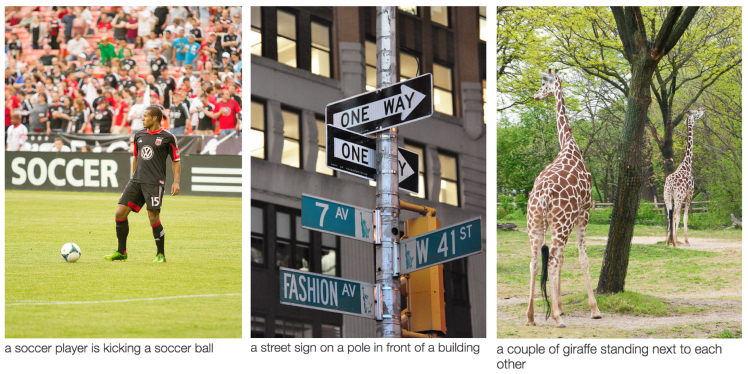
\includegraphics[width=0.8\linewidth,keepaspectratio]{cnn1}
\end{center}

 \begin{itemize}
\item  ConvNet is able to recognize scenes and the system is able to suggest relevant captions (``a soccer player is kicking a soccer ball'')
\item Also, being used for recognizing everyday objects, humans and animals.
\end{itemize}
\end{frame}


%%%%%%%%%%%%%%%%%%%%%%%%%%%%%%%%%%%%%%%%%%%%%%%%%%%
\begin{frame}[fragile] \frametitle{What is CNN?}

\begin{itemize}
\item Inspired by mammalian visual cortex.
\item The visual cortex contains a complex arrangement of cells
\item Sensitive to small sub-regions of the visual field, 
\item Cells act as local filters over the input space.
\end{itemize}
\end{frame}

%%%%%%%%%%%%%%%%%%%%%%%%%%%%%%%%%%%%%%%%%%%%%%%%%%%
\begin{frame}[fragile] \frametitle{What is CNN?}

Different filter/cell types
\begin{itemize}
\item Simple cells respond maximally to specific edge-like patterns.
\item Complex cells have larger receptive fields and are locally invariant to position.

\end{itemize}
\end{frame}



%%%%%%%%%%%%%%%%%%%%%%%%%%%%%%%%%%%%%%%%%%%%%%%%%%%
\begin{frame}
  \begin{center}
    {\Large CNN History}
  \end{center}
\end{frame}





%%%%%%%%%%%%%%%%%%%%%%%%%%%%%%%%%%%%%%%%%%%%%%%%%%%
\begin{frame}[fragile] \frametitle{History}


\begin{itemize}
\item LeNet Architecture (1990s): Pioneering work by Yann LeCun was named LeNet5 after many previous successful iterations since the year 1988 
\item Used mainly for character recognition tasks such as reading zip codes, digits, etc.

\end{itemize}
\end{frame}

%%%%%%%%%%%%%%%%%%%%%%%%%%%%%%%%%%%%%%%%%%%%%%%%%%%
\begin{frame}[fragile] \frametitle{History}
There have been several new architectures proposed in the recent years which are improvements over the LeNet, but they all use the main concepts from the LeNet and are relatively easier to understand.

\begin{center}
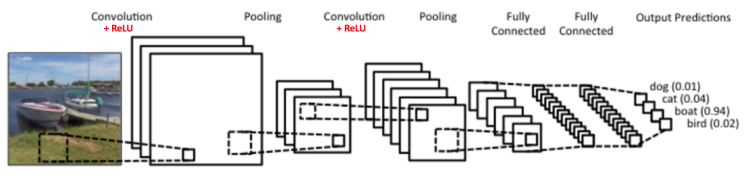
\includegraphics[width=0.8\linewidth,keepaspectratio]{cnn2}
\end{center}
On receiving a boat image as input, the network correctly assigns the highest probability for boat (0.94) among all four categories. 
\end{frame}

%%%%%%%%%%%%%%%%%%%%%%%%%%%%%%%%%%%%%%%%%%%%%%%%%%%
\begin{frame}[fragile] \frametitle{Concept}
There are four main operations in the ConvNet 

\begin{itemize}
\item Convolution
\item Non Linearity (ReLU)
\item Pooling or Sub Sampling
\item Classification (Fully Connected Layer)
\end{itemize}
\end{frame}



%%%%%%%%%%%%%%%%%%%%%%%%%%%%%%%%%%%%%%%%%%%%%%%%%%%
\begin{frame}
  \begin{center}
    {\Large CNN Example}
  \end{center}
\end{frame}

%%%%%%%%%%%%%%%%%%%%%%%%%%%%%%%%%%%%%%%%%%%%%%%%%%%
\begin{frame}[fragile] \frametitle{Images}
Simplification: Assuming only 0 and 1 (black or white) are the values, here is the representation of a smiley image:

\begin{center}
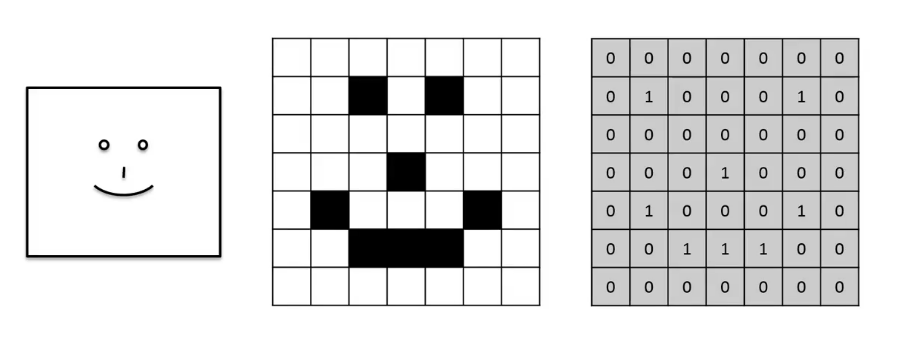
\includegraphics[width=0.8\linewidth,keepaspectratio]{cnn43}

\tiny{(Ref: Deep Learning A-Z - Kirill Eremenko)}
\end{center}



\end{frame}



%%%%%%%%%%%%%%%%%%%%%%%%%%%%%%%%%%%%%%%%%%%%%%%%%%%
\begin{frame}[fragile] \frametitle{Images}

\begin{center}
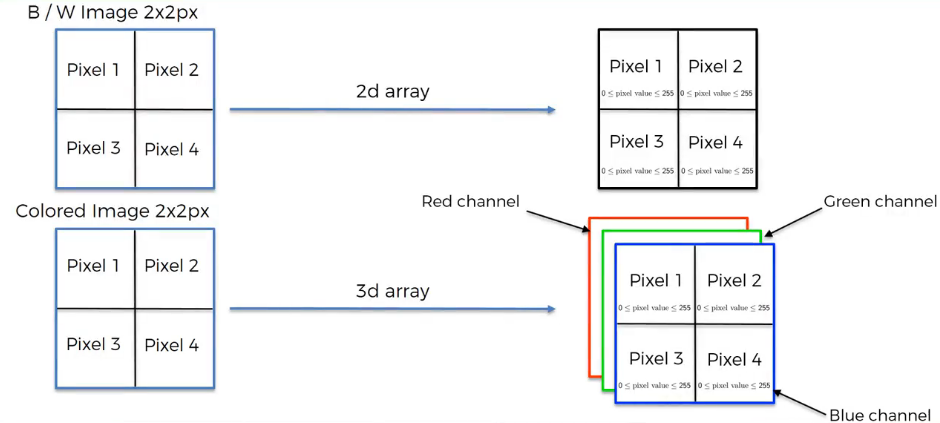
\includegraphics[width=0.8\linewidth,keepaspectratio]{cnn42}

\tiny{(Ref: Deep Learning A-Z - Kirill Eremenko)}
\end{center}

\begin{itemize}
\item For Grey scale image, each pixel has value from 0 (black) to 255 (white), $2^8$ as its 8 bit.
\item For Color image, there are 3 such matrices, one each for Red Green Blue.
\end{itemize}


\end{frame}

%%%%%%%%%%%%%%%%%%%%%%%%%%%%%%%%%%%%%%%%%%%%%%%%%%%
\begin{frame}[fragile] \frametitle{Step 1 : Convolution}

\begin{center}
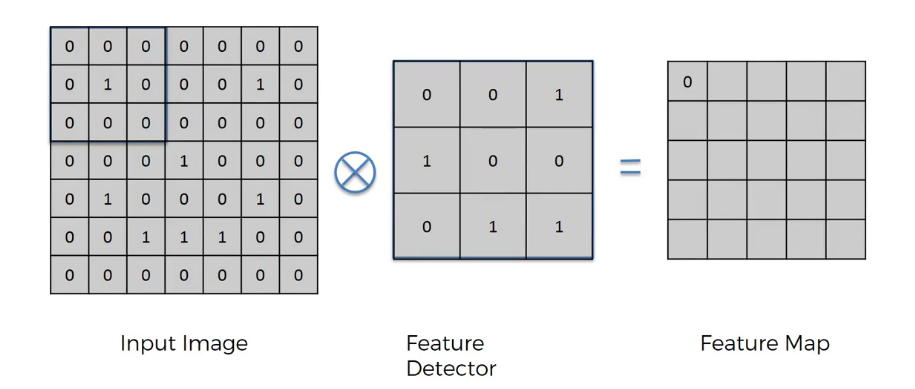
\includegraphics[width=0.8\linewidth,keepaspectratio]{cnn45}

\tiny{(Ref: Deep Learning A-Z - Kirill Eremenko)}
\end{center}

\begin{itemize}
\item Feature detector, same as filter, or convolution operator.
\item Traverse the Input Image using Feature Detector, doing dot product at each position, then storing result in the ``feature map''.
\item The amount of movement is called ``stride''.
\end{itemize}
\end{frame}

%%%%%%%%%%%%%%%%%%%%%%%%%%%%%%%%%%%%%%%%%%%%%%%%%%%
\begin{frame}[fragile] \frametitle{Step 1 : Convolution}

\begin{center}
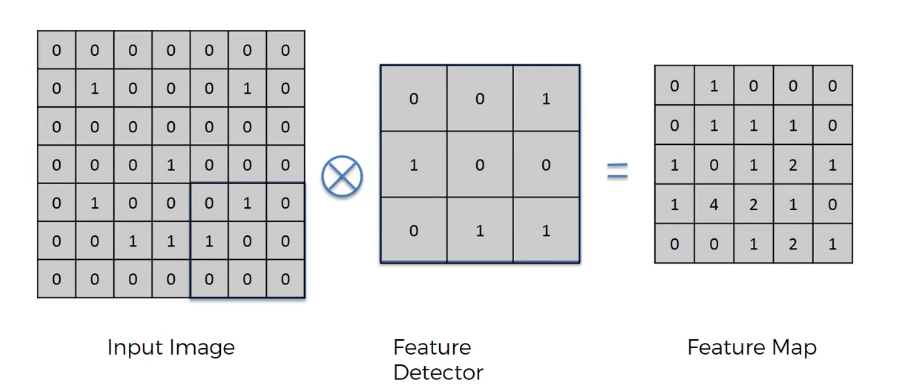
\includegraphics[width=0.8\linewidth,keepaspectratio]{cnn46}

\tiny{(Ref: Deep Learning A-Z - Kirill Eremenko)}
\end{center}

What have we done?:
\begin{itemize}
\item Reduced the image size. More with bigger stride.
\item Finally we want to go up to few enum values, for classification.
\item While doing this dimension reduction, we wish to store the aggregated information.
\item Some info is lost, but the relevant info (around features) is kept or even enhanced (``4'' in the output).
\end{itemize}

\end{frame}

%%%%%%%%%%%%%%%%%%%%%%%%%%%%%%%%%%%%%%%%%%%%%%%%%%%
\begin{frame}[fragile] \frametitle{Step 1 : Convolution}

\begin{center}
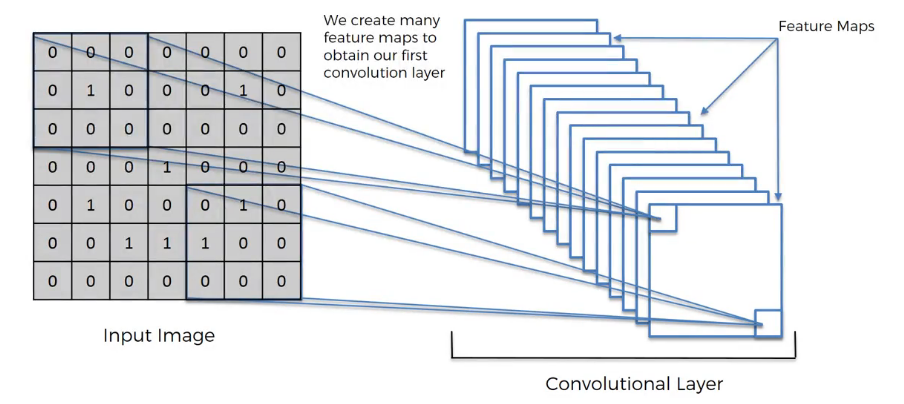
\includegraphics[width=0.8\linewidth,keepaspectratio]{cnn47}

\tiny{(Ref: Deep Learning A-Z - Kirill Eremenko)}
\end{center}

\begin{itemize}
\item We as humans do not look at each pixel, but at strong features.
\item We use multiple feature maps to accentuate multiple features.
\end{itemize}

\end{frame}

%%%%%%%%%%%%%%%%%%%%%%%%%%%%%%%%%%%%%%%%%%%%%%%%%%%
\begin{frame}[fragile] \frametitle{Filter for Sharpen}
Experimentation: Using GIMP to apply filters on an image of Taj Mahal

\begin{center}
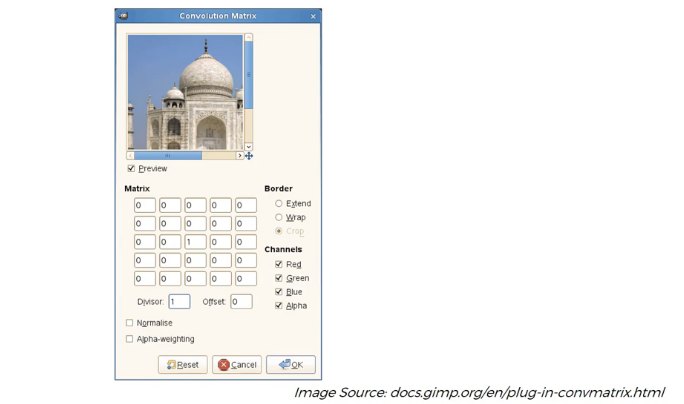
\includegraphics[width=0.8\linewidth,keepaspectratio]{cnn48}

\tiny{(Ref: Deep Learning A-Z - Kirill Eremenko)}
\end{center}

\end{frame}

%%%%%%%%%%%%%%%%%%%%%%%%%%%%%%%%%%%%%%%%%%%%%%%%%%%
\begin{frame}[fragile] \frametitle{Filter for Sharpen}

\begin{center}
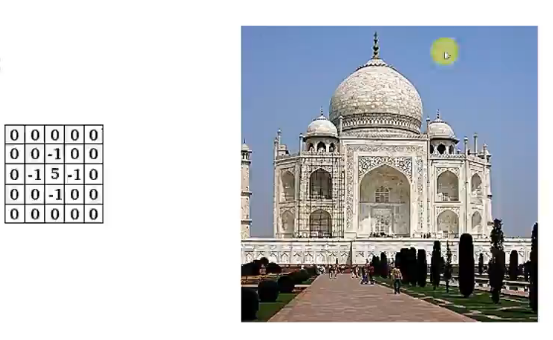
\includegraphics[width=0.8\linewidth,keepaspectratio]{cnn49}

\tiny{(Ref: Deep Learning A-Z - Kirill Eremenko)}
\end{center}

``5'' is in the middle of the filter and surroundings are ``-1''.  It enhances center and reduces neighbors. Thus sharpens.
Imp to note that it does not shuffle the pixels, so, preserves the pattern.
\end{frame}

%%%%%%%%%%%%%%%%%%%%%%%%%%%%%%%%%%%%%%%%%%%%%%%%%%%
\begin{frame}[fragile] \frametitle{Filter for Blurr}

\begin{center}
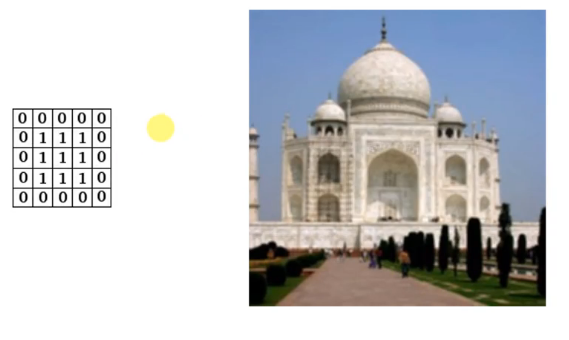
\includegraphics[width=0.8\linewidth,keepaspectratio]{cnn50}

\tiny{(Ref: Deep Learning A-Z - Kirill Eremenko)}
\end{center}

\end{frame}

%%%%%%%%%%%%%%%%%%%%%%%%%%%%%%%%%%%%%%%%%%%%%%%%%%%
\begin{frame}[fragile] \frametitle{Filter for Edge Detect}

\begin{center}
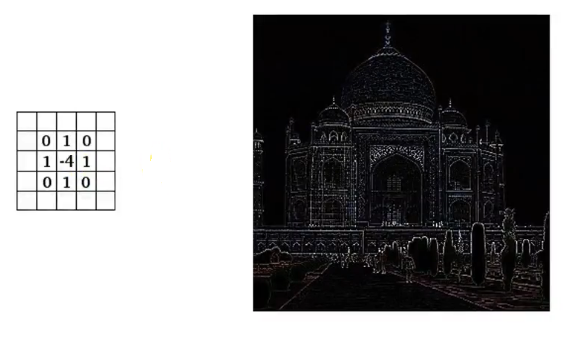
\includegraphics[width=0.8\linewidth,keepaspectratio]{cnn51}

\tiny{(Ref: Deep Learning A-Z - Kirill Eremenko)}
\end{center}

\end{frame}

%%%%%%%%%%%%%%%%%%%%%%%%%%%%%%%%%%%%%%%%%%%%%%%%%%%
\begin{frame}[fragile] \frametitle{Filter for Emboss}

\begin{center}
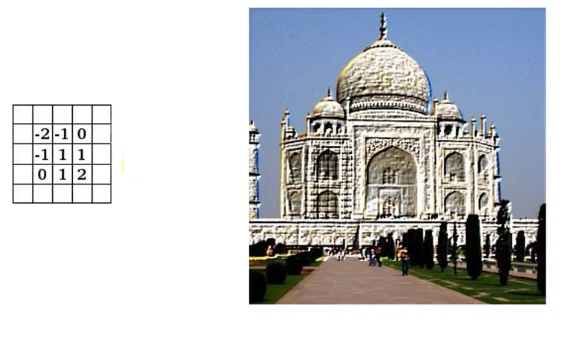
\includegraphics[width=0.8\linewidth,keepaspectratio]{cnn52}

\tiny{(Ref: Deep Learning A-Z - Kirill Eremenko)}
\end{center}

\end{frame}

%%%%%%%%%%%%%%%%%%%%%%%%%%%%%%%%%%%%%%%%%%%%%%%%%%%
\begin{frame}[fragile] \frametitle{Step 1B : Relu}

\begin{center}
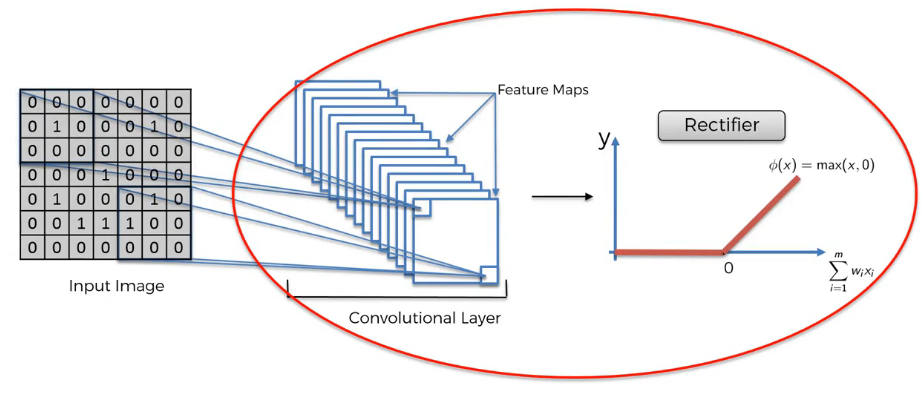
\includegraphics[width=0.8\linewidth,keepaspectratio]{cnn53}

\tiny{(Ref: Deep Learning A-Z - Kirill Eremenko)}
\end{center}

 Increases non linearity (as image itself are not linearly progressing).


\end{frame}


%%%%%%%%%%%%%%%%%%%%%%%%%%%%%%%%%%%%%%%%%%%%%%%%%%%
\begin{frame}[fragile] \frametitle{Step 1B : Relu}

\begin{center}
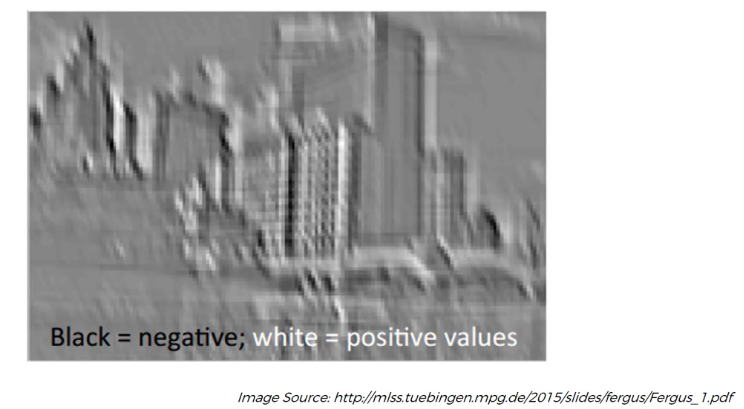
\includegraphics[width=0.45\linewidth,keepaspectratio]{cnn54}
\end{center}

\begin{itemize}
\item Just using Feature Detector gives above output.
\item ReLu makes it non negative, as shown below. Introduces non-linearity.
\end{itemize}


\begin{center}
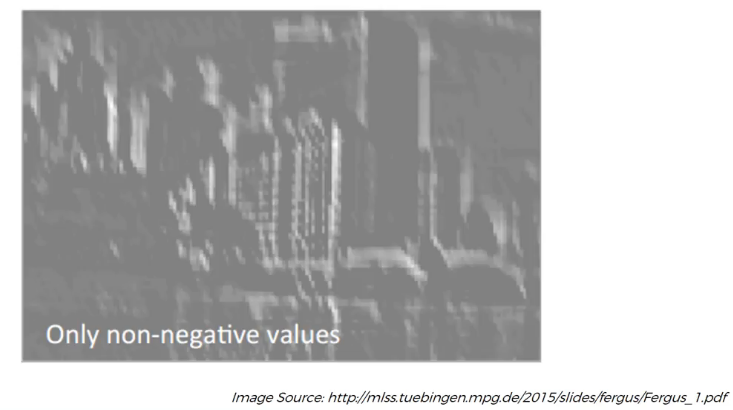
\includegraphics[width=0.45\linewidth,keepaspectratio]{cnn55}
\end{center}
\end{frame}

%%%%%%%%%%%%%%%%%%%%%%%%%%%%%%%%%%%%%%%%%%%%%%%%%%%
\begin{frame}[fragile] \frametitle{Step 2 : Max Pooling}

\begin{center}
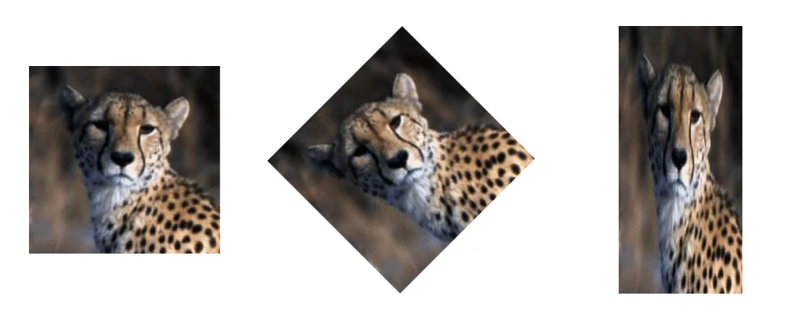
\includegraphics[width=0.8\linewidth,keepaspectratio]{cnn56}

\tiny{(Ref: Deep Learning A-Z - Kirill Eremenko)}
\end{center}

\begin{itemize}
\item Images can be transformed: scaled, rotated.
\item But you need to identify each as the same.
\item So, if you take MAX values, it does not matter its location in the image.
\end{itemize}

\end{frame}

%%%%%%%%%%%%%%%%%%%%%%%%%%%%%%%%%%%%%%%%%%%%%%%%%%%
\begin{frame}[fragile] \frametitle{Step 2 : Max Pooling}

\begin{center}
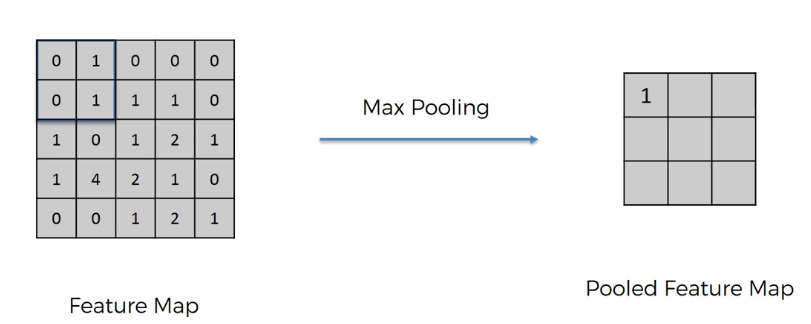
\includegraphics[width=0.8\linewidth,keepaspectratio]{cnn57}

\tiny{(Ref: Deep Learning A-Z - Kirill Eremenko)}
\end{center}

\begin{itemize}
\item A smaller window (not filter), use MAX of the window and dis regard other 3. 
\item No DOT product here.
\item Good reduction in dimension.
\item There are other types of pooling to ``reduce', like average pooling.
\end{itemize}

\end{frame}

%%%%%%%%%%%%%%%%%%%%%%%%%%%%%%%%%%%%%%%%%%%%%%%%%%%
\begin{frame}[fragile] \frametitle{Visualization Tool}


\begin{center}
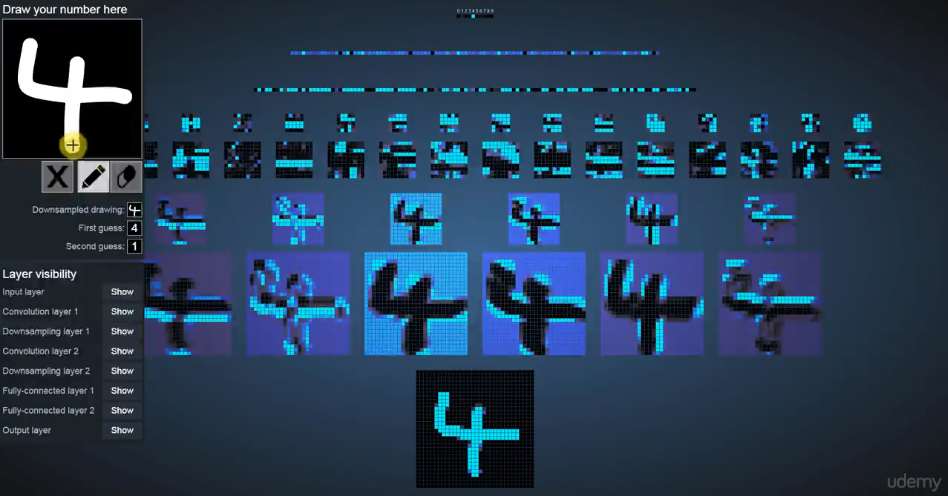
\includegraphics[width=0.8\linewidth,keepaspectratio]{cnn58}

\tiny{(Ref: Deep Learning A-Z - Kirill Eremenko)}
\end{center}

Adam Harley: http://scs.ryerson.ca/~aharley/vis/conv/

Draw an image and it shows (bottom to top) CNN layers.

\end{frame}

%%%%%%%%%%%%%%%%%%%%%%%%%%%%%%%%%%%%%%%%%%%%%%%%%%%
\begin{frame}[fragile] \frametitle{Step 3 : Flattening}

\begin{center}
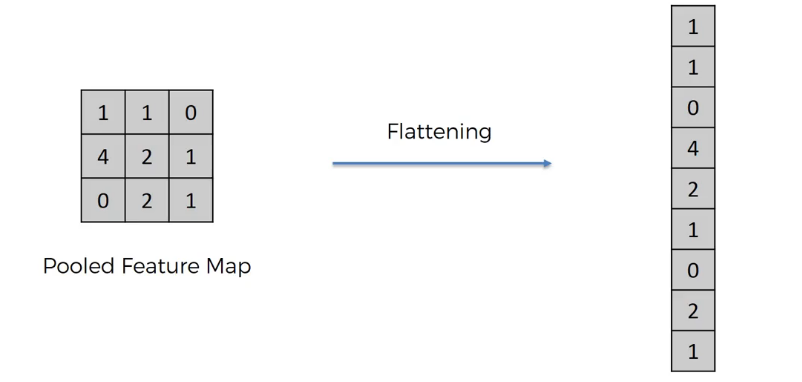
\includegraphics[width=0.8\linewidth,keepaspectratio]{cnn59}

\tiny{(Ref: Deep Learning A-Z - Kirill Eremenko)}
\end{center}

\begin{itemize}
\item Just making a vector out of matrix, so that it becomes in put to the new layer.
\item Each filter will give its own vector, all such vectors can be clubbed together in a single column vector.
\end{itemize}

\end{frame}

%%%%%%%%%%%%%%%%%%%%%%%%%%%%%%%%%%%%%%%%%%%%%%%%%%%
\begin{frame}[fragile] \frametitle{Step 4 : Full Connection}

\begin{center}
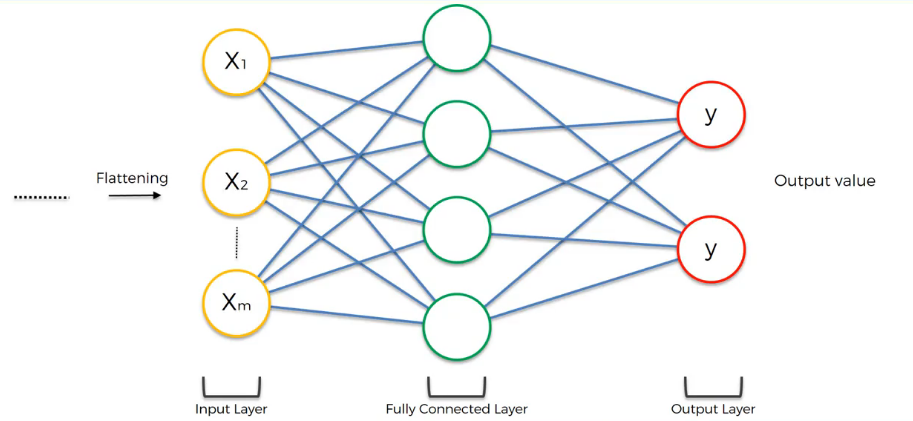
\includegraphics[width=0.8\linewidth,keepaspectratio]{cnn60}

\tiny{(Ref: Deep Learning A-Z - Kirill Eremenko)}
\end{center}

\begin{itemize}
\item Adding NN after inputs are ready from previous step
\item Fully connected network for classification
\end{itemize}

\end{frame}

%%%%%%%%%%%%%%%%%%%%%%%%%%%%%%%%%%%%%%%%%%%%%%%%%%%
\begin{frame}[fragile] \frametitle{Step 4 : Full Connection}

\begin{center}
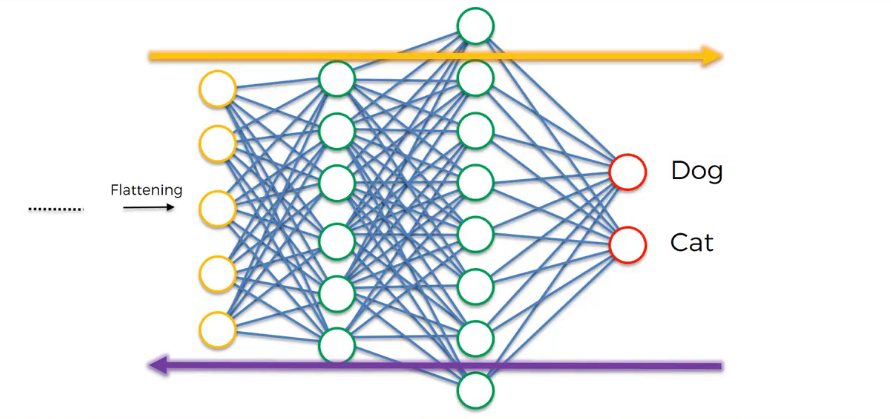
\includegraphics[width=0.8\linewidth,keepaspectratio]{cnn61}

\tiny{(Ref: Deep Learning A-Z - Kirill Eremenko)}
\end{center}

\begin{itemize}
\item For binary output, single output is ok, but for multi class , those many output nodes are needed.
\item In back propagation both, NN weights as well as Feature detector values are adjusted.

\end{itemize}

\end{frame}

%%%%%%%%%%%%%%%%%%%%%%%%%%%%%%%%%%%%%%%%%%%%%%%%%%%
\begin{frame}[fragile] \frametitle{Step 4 : Full Connection}

\begin{center}
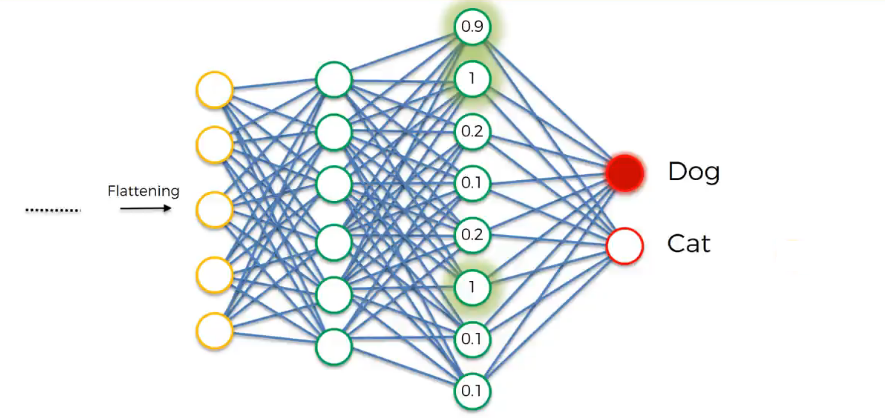
\includegraphics[width=0.8\linewidth,keepaspectratio]{cnn62}

\tiny{(Ref: Deep Learning A-Z - Kirill Eremenko)}
\end{center}

\begin{itemize}
\item At the last hidden layer, we have float values.
\item All the values are common to both nodes.
\item The blue line weights, during training, get adjusted so that probability of specific output is adjusted properly.

\end{itemize}

\end{frame}

%%%%%%%%%%%%%%%%%%%%%%%%%%%%%%%%%%%%%%%%%%%%%%%%%%%
\begin{frame}[fragile] \frametitle{Step 4 : Full Connection}

\begin{center}
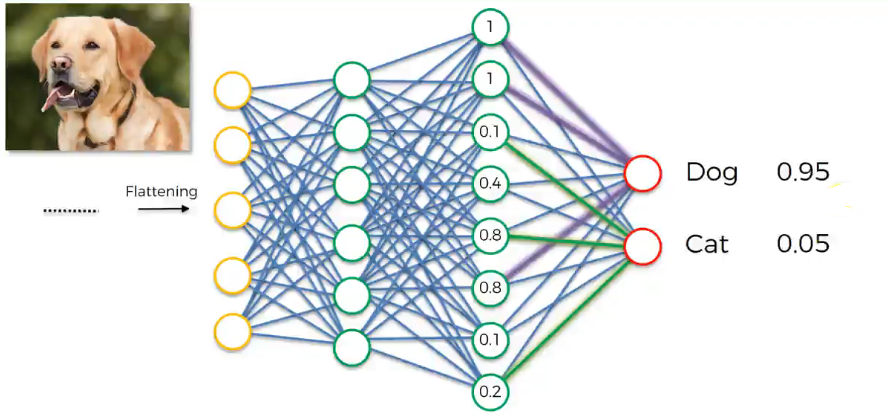
\includegraphics[width=0.8\linewidth,keepaspectratio]{cnn63}

\tiny{(Ref: Deep Learning A-Z - Kirill Eremenko)}
\end{center}

Trained model can then be used for predictions.
\end{frame}


%%%%%%%%%%%%%%%%%%%%%%%%%%%%%%%%%%%%%%%%%%%%%%%%%%%
\begin{frame}[fragile] \frametitle{Softmax}

Softmax converts array of floats to probabilities, adding to 1. Look at denominattor, its sum of all probabilitites.

\begin{center}
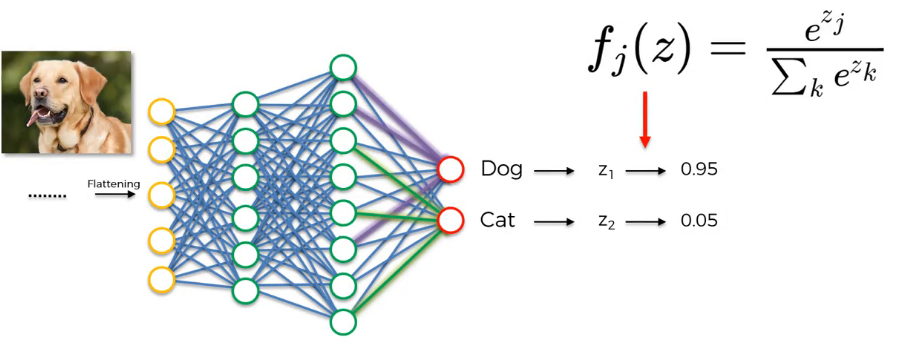
\includegraphics[width=0.8\linewidth,keepaspectratio]{cnn65}

\tiny{(Ref: Deep Learning A-Z - Kirill Eremenko)}
\end{center}


\end{frame}

%%%%%%%%%%%%%%%%%%%%%%%%%%%%%%%%%%%%%%%%%%%%%%%%%%%
\begin{frame}[fragile] \frametitle{Cross Entropy}

Cross Entropy is loss function. Looks very similar to loss function in Logistic Regression.

\begin{center}
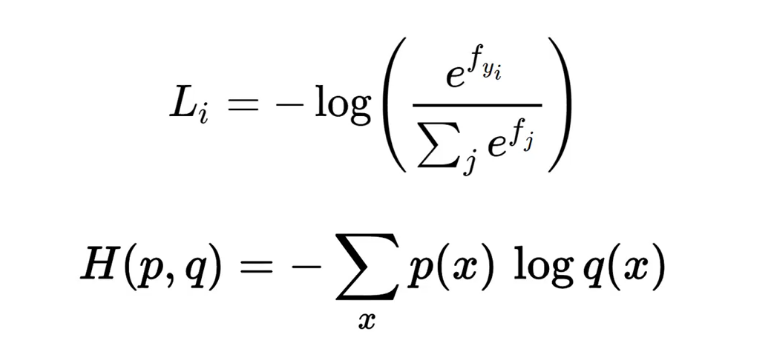
\includegraphics[width=0.8\linewidth,keepaspectratio]{cnn66}

\tiny{(Ref: Deep Learning A-Z - Kirill Eremenko)}
\end{center}


\end{frame}


%%%%%%%%%%%%%%%%%%%%%%%%%%%%%%%%%%%%%%%%%%%%%%%%%%%
\begin{frame}[fragile] \frametitle{Loss Function}

During training, loss can be calculated. p is actual value, whereas q is predicted value.

\begin{center}
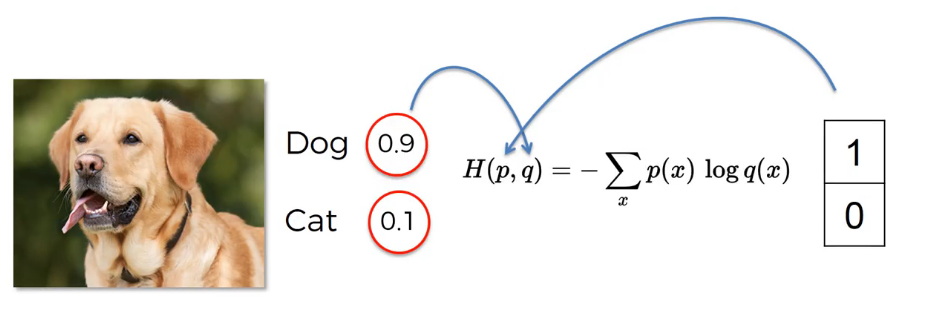
\includegraphics[width=0.8\linewidth,keepaspectratio]{cnn67}

\tiny{(Ref: Deep Learning A-Z - Kirill Eremenko)}
\end{center}

Loss is minimized by adusting weights in NN as well as filter values.
\end{frame}


%%%%%%%%%%%%%%%%%%%%%%%%%%%%%%%%%%%%%%%%%%%%%%%%%%%
\begin{frame}[fragile] \frametitle{Performance Comparison}

Follwoing is data for two CNNs.

\begin{center}
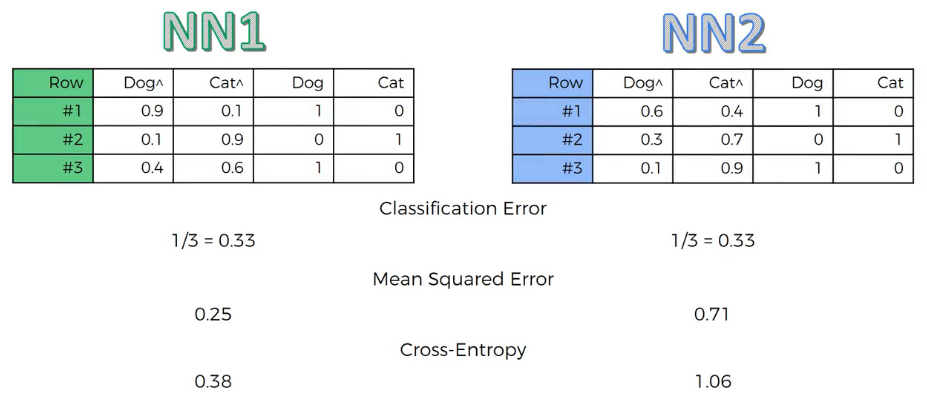
\includegraphics[width=0.8\linewidth,keepaspectratio]{cnn68}

\tiny{(Ref: Deep Learning A-Z - Kirill Eremenko)}
\end{center}

Each of them got 1/3 wrong. So, accuracy wise they are same. Cross entropy is better than MSE as, due to log, it works well with smaller values.
\end{frame}



%%%%%%%%%%%%%%%%%%%%%%%%%%%%%%%%%%%%%%%%%%%%%%%%%%%
\begin{frame}[fragile] \frametitle{Summary}

\begin{center}
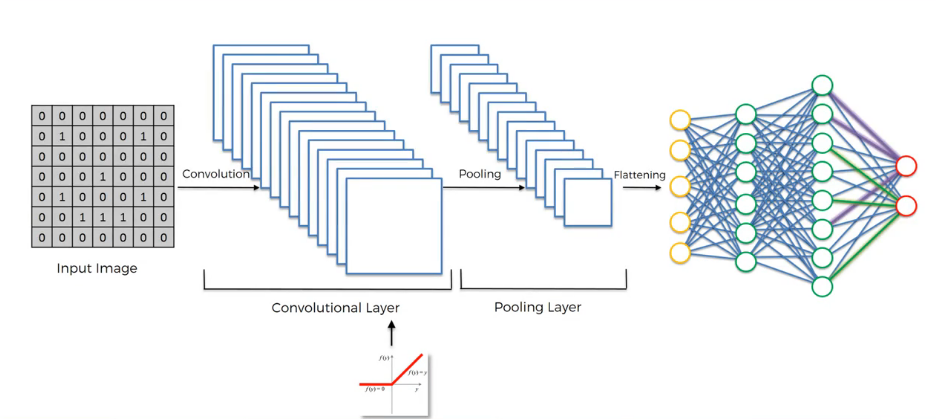
\includegraphics[width=0.8\linewidth,keepaspectratio]{cnn64}

\tiny{(Ref: Deep Learning A-Z - Kirill Eremenko)}
\end{center}

\end{frame}

%%%%%%%%%%%%%%%%%%%%%%%%%%%%%%%%%%%%%%%%%%%%%%%%%%%
\begin{frame}[fragile] \frametitle{Are filters also optimized during Back-propagation?}

\begin{itemize}
\item  We don't know upfront what the filters are needed for any given problem. 
\item They get set automatically through the back-propagation procedure. 
\item Values inside each filter get updated along with other weights and biases.
\end{itemize}

\tiny{(Ref: How filters are made in a CNN? - Stack Overflow)}
\end{frame}

% %%%%%%%%%%%%%%%%%%%%%%%%%%%%%%%%%%%%%%%%%%%%%%%%%%%
% \begin{frame}
  % \begin{center}
    % {\Large Toy Example: Image Recognition Classifier (Ref: Luis Serrano)}
  % \end{center}
% \end{frame}

% %%%%%%%%%%%%%%%%%%%%%%%%%%%%%%%%%%%%%%%%%%%%%%%%%%%
% \begin{frame}[fragile] \frametitle{Image Recognition Classifier }
% \begin{itemize}
% \item  We have only 2x2 images. One for ``\textbackslash'' and another for ``/'''
% \item Highly pixeleted lines.
% \item So they are 2x2 matrices with -1 for white and +1 for color.
% \item We read them as linear array.
% \end{itemize}
% \begin{center}
% 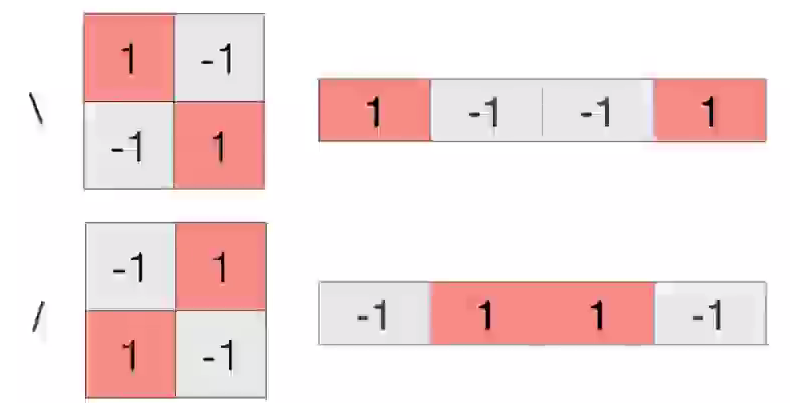
\includegraphics[width=0.6\linewidth,keepaspectratio]{cnn16}
% \end{center}
% \end{frame}


% %%%%%%%%%%%%%%%%%%%%%%%%%%%%%%%%%%%%%%%%%%%%%%%%%%%
% \begin{frame}[fragile] \frametitle{Toy Example: Image Recognition Classifier}

 % \begin{itemize}
% \item How can you tell them apart?
% \item One way: add them together does not differentiate
% \item Another way: Multiplying them also does not differentiate
% \item Which Operation to use?
% \end{itemize}

% \begin{center}
% 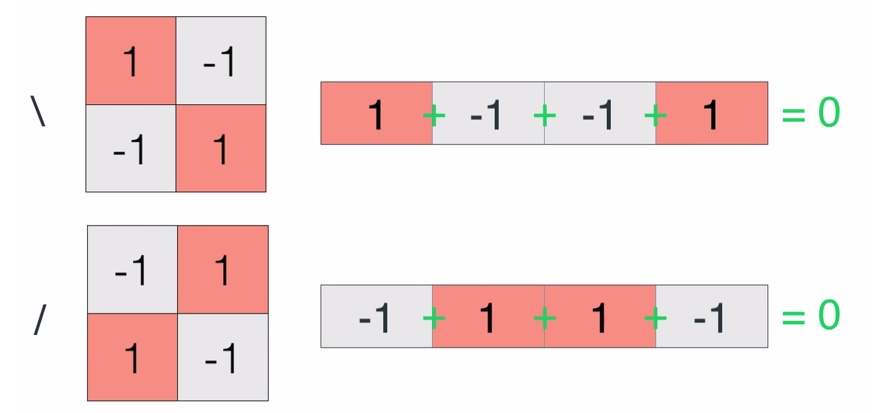
\includegraphics[width=\linewidth,keepaspectratio]{cnn17}
% \end{center}
% \end{frame}


% %%%%%%%%%%%%%%%%%%%%%%%%%%%%%%%%%%%%%%%%%%%%%%%%%%%
% \begin{frame}[fragile] \frametitle{Toy Example: Image Recognition Classifier}

 % \begin{itemize}
% \item Assign operation to each cell position
% \item Multiplying and adding them differentiates!!
% \item Our First Image Classifier!!!
% \end{itemize}
% \begin{center}
% 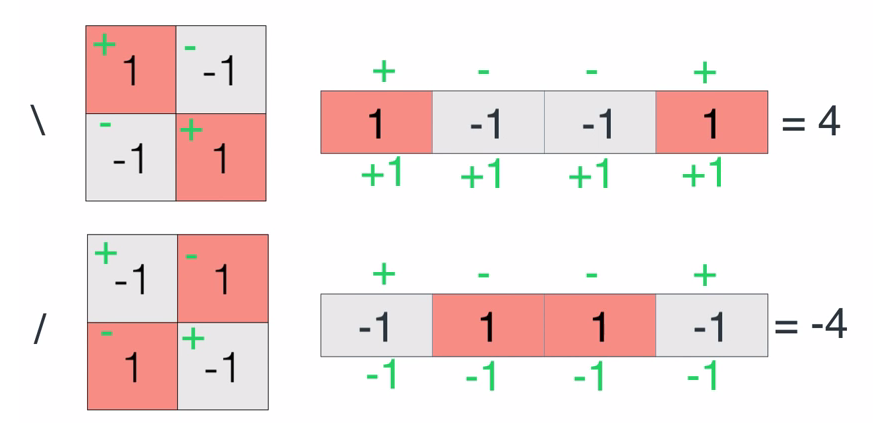
\includegraphics[width=\linewidth,keepaspectratio]{cnn18}
% \end{center}
% \end{frame}

% %%%%%%%%%%%%%%%%%%%%%%%%%%%%%%%%%%%%%%%%%%%%%%%%%%%
% \begin{frame}[fragile] \frametitle{Toy Example: Image Recognition Classifier}
 % \begin{itemize}
% \item Using square box tool
% \item Which overlaps, and computes a number
% \end{itemize}
% \begin{center}
% 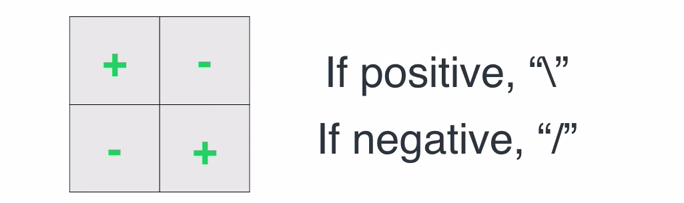
\includegraphics[width=\linewidth,keepaspectratio]{cnn19}
% \end{center}
% \end{frame}

% %%%%%%%%%%%%%%%%%%%%%%%%%%%%%%%%%%%%%%%%%%%%%%%%%%%
% \begin{frame}[fragile] \frametitle{Toy Example: Image Recognition Classifier}
 % \begin{itemize}
% \item Top one looks like badly drawn backward slash
% \item Bottom one is sort of a forward slash
% \item Still it tells them apart and with ok result
% \end{itemize}
% \begin{center}
% 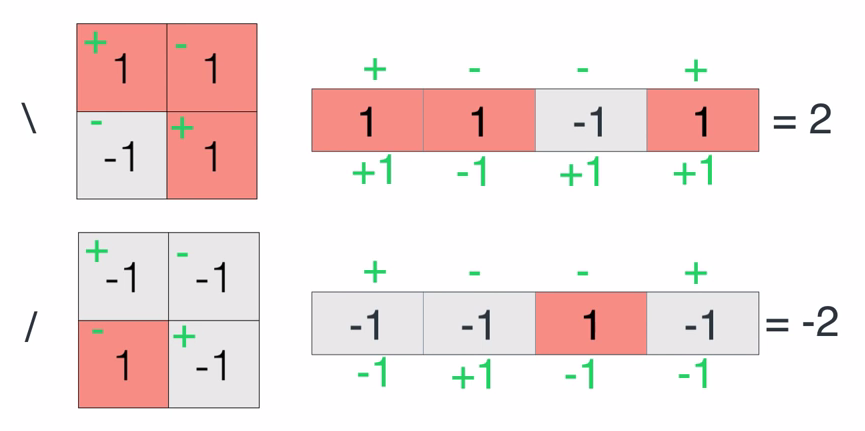
\includegraphics[width=0.6\linewidth,keepaspectratio]{cnn20}
% \end{center}
% \end{frame}

% %%%%%%%%%%%%%%%%%%%%%%%%%%%%%%%%%%%%%%%%%%%%%%%%%%%
% \begin{frame}[fragile] \frametitle{Toy Example: Image Recognition Classifier}
 % \begin{itemize}
% \item Can we come up with the good square box?
% \item Well, we try all permutations and see if we can differentiate well, with the labelled data
% \item With just 2x2 box there are 16 choices. 
% \item For larger size, it could be huge.
% \end{itemize}
% \begin{center}
% 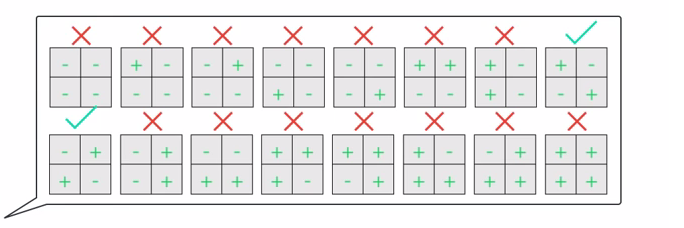
\includegraphics[width=\linewidth,keepaspectratio]{cnn21}
% \end{center}
% \end{frame}

% %%%%%%%%%%%%%%%%%%%%%%%%%%%%%%%%%%%%%%%%%%%%%%%%%%%
% \begin{frame}[fragile] \frametitle{Toy Example: Image Recognition Classifier}
 % \begin{itemize}
% \item In practice we don't enumerate all
% \item We start with a random and go on changing a bit to get to a good box.
% \item Similar to Gradient descent
% \end{itemize}
% \begin{center}
% 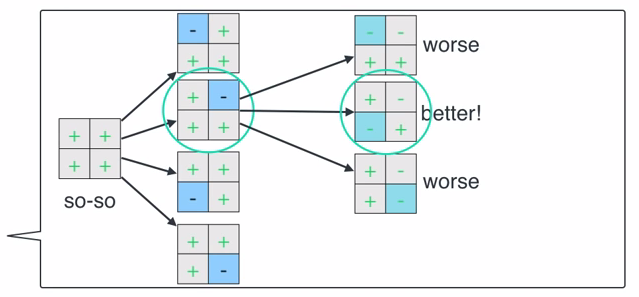
\includegraphics[width=\linewidth,keepaspectratio]{cnn22}
% \end{center}
% \end{frame}


% %%%%%%%%%%%%%%%%%%%%%%%%%%%%%%%%%%%%%%%%%%%%%%%%%%%
% \begin{frame}[fragile] \frametitle{Toy Example: Image Recognition Classifier}
 % \begin{itemize}
% \item If we have 3x3 we can classify 4 figures.
% \item We can use previous idea and combine
% \end{itemize}
% \begin{center}
% 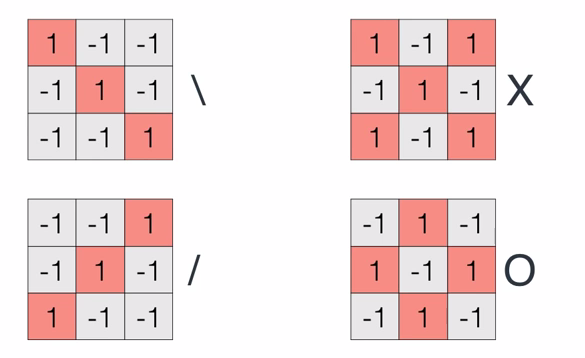
\includegraphics[width=\linewidth,keepaspectratio]{cnn23}
% \end{center}
% \end{frame}

% %%%%%%%%%%%%%%%%%%%%%%%%%%%%%%%%%%%%%%%%%%%%%%%%%%%
% \begin{frame}[fragile] \frametitle{Toy Example: Image Recognition Classifier}
% Fit 2x2 at all places and output its corresponding forward or backward slash (in the middle layer)
% \begin{center}
% 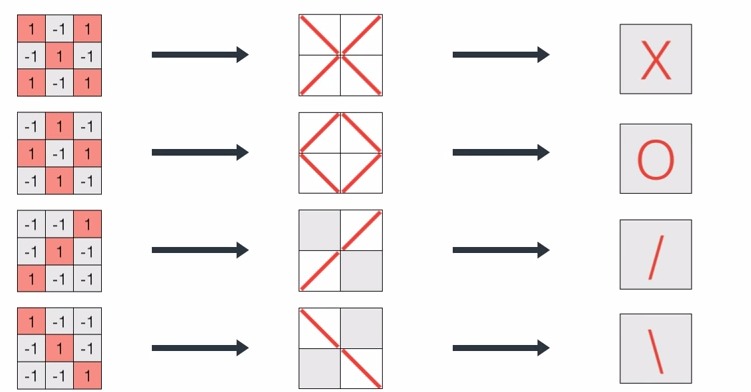
\includegraphics[width=\linewidth,keepaspectratio]{cnn24}
% \end{center}
% \end{frame}

% %%%%%%%%%%%%%%%%%%%%%%%%%%%%%%%%%%%%%%%%%%%%%%%%%%%
% \begin{frame}[fragile] \frametitle{Toy Example: Image Recognition Classifier}
 % \begin{itemize}
% \item Convolution breaks the image and computes intermediate results
% \item Final fully connected layer, combines to form meaningful output
% \end{itemize}
% \begin{center}
% 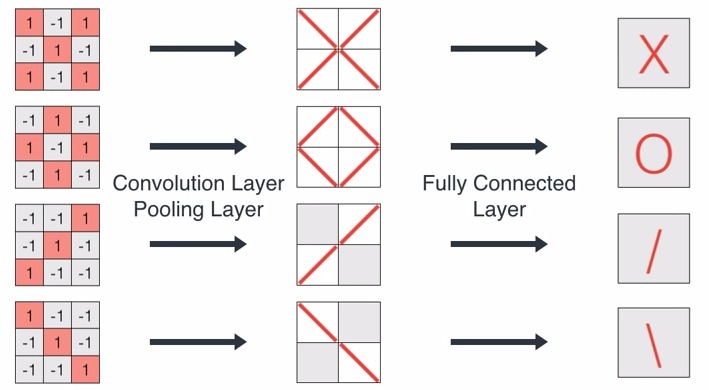
\includegraphics[width=0.8\linewidth,keepaspectratio]{cnn25}
% \end{center}
% \end{frame}

% %%%%%%%%%%%%%%%%%%%%%%%%%%%%%%%%%%%%%%%%%%%%%%%%%%%
% \begin{frame}[fragile] \frametitle{Toy Example: Image Recognition Classifier}
 % \begin{itemize}
% \item  Square boxes are called filters
% \item They overlap and slide
% \item At each position they compute and put result 4
% \item 4 being more than threshold, put the backward slash. and so on.
% \end{itemize}
% \begin{center}
% 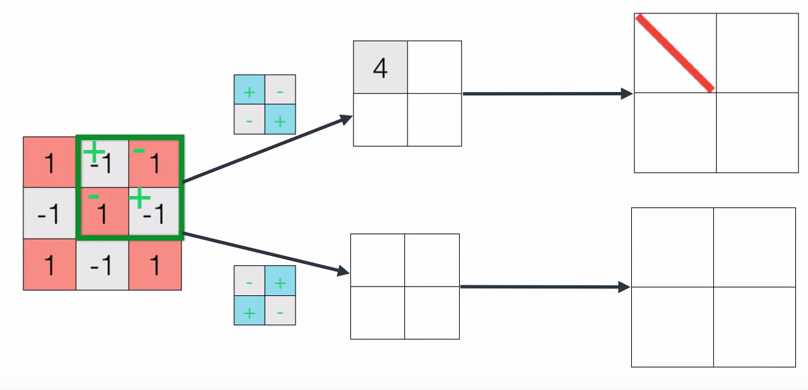
\includegraphics[width=\linewidth,keepaspectratio]{cnn26}
% \end{center}
% \end{frame}

% %%%%%%%%%%%%%%%%%%%%%%%%%%%%%%%%%%%%%%%%%%%%%%%%%%%
% \begin{frame}[fragile] \frametitle{Toy Example: Image Recognition Classifier}
 % \begin{itemize}
% \item  When sliding is over, we get the backward slash
% \item Do the same with another filter
% \end{itemize}
% \begin{center}
% 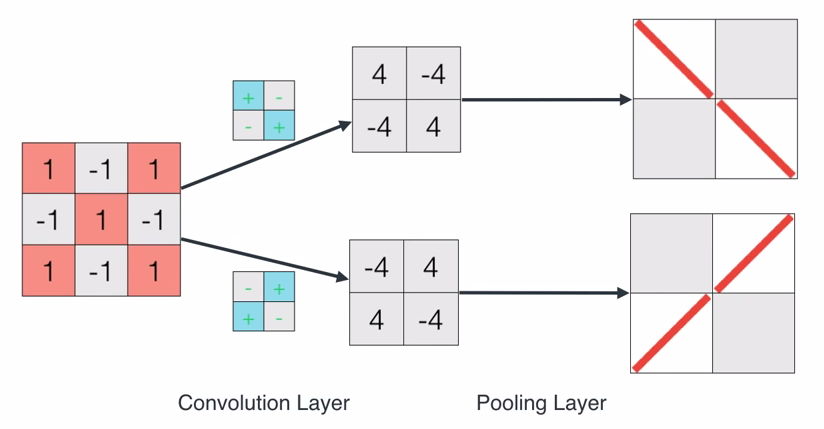
\includegraphics[width=\linewidth,keepaspectratio]{cnn27}
% \end{center}
% \end{frame}

% %%%%%%%%%%%%%%%%%%%%%%%%%%%%%%%%%%%%%%%%%%%%%%%%%%%
% \begin{frame}[fragile] \frametitle{Toy Example: Image Recognition Classifier}
 % \begin{itemize}
% \item  Final layer combines them
% \item To form the X
% \end{itemize}
% \begin{center}
% 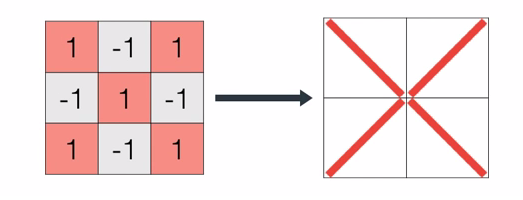
\includegraphics[width=\linewidth,keepaspectratio]{cnn28}
% \end{center}
% \end{frame}

% %%%%%%%%%%%%%%%%%%%%%%%%%%%%%%%%%%%%%%%%%%%%%%%%%%%
% \begin{frame}[fragile] \frametitle{Toy Example: Image Recognition Classifier}
% O
% \begin{center}
% 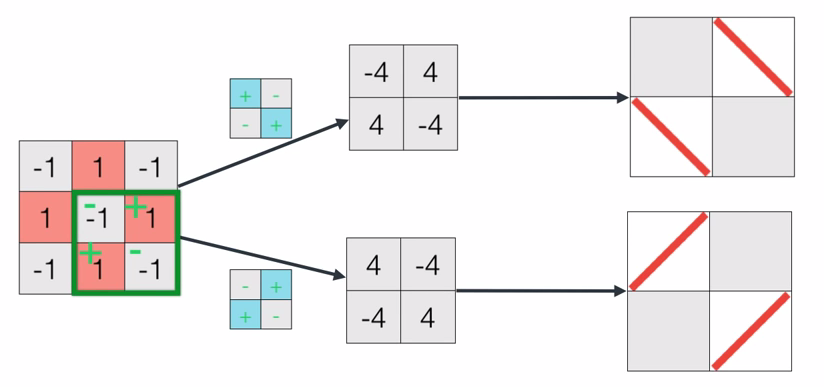
\includegraphics[width=\linewidth,keepaspectratio]{cnn29}
% \end{center}
% \end{frame}

% %%%%%%%%%%%%%%%%%%%%%%%%%%%%%%%%%%%%%%%%%%%%%%%%%%%
% \begin{frame}[fragile] \frametitle{Toy Example: Image Recognition Classifier}
% \
% \begin{center}
% 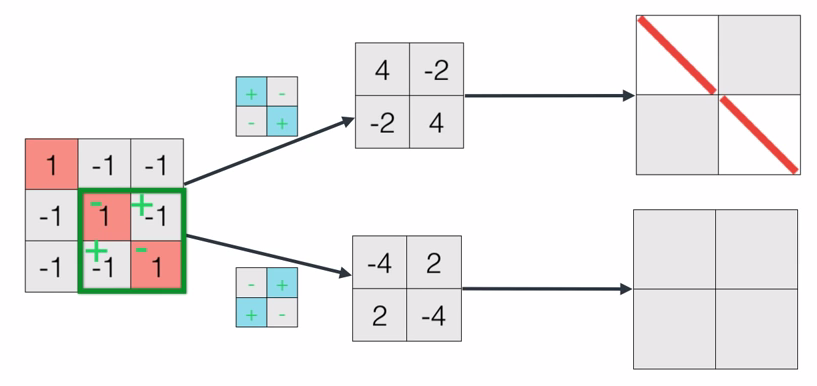
\includegraphics[width=\linewidth,keepaspectratio]{cnn30}
% \end{center}
% \end{frame}

% %%%%%%%%%%%%%%%%%%%%%%%%%%%%%%%%%%%%%%%%%%%%%%%%%%%
% \begin{frame}[fragile] \frametitle{Toy Example: Image Recognition Classifier}
% How to collect pooled outputs?
 % \begin{itemize}
% \item  Reads outputs are a list (array)
% \item There are two basis, ie forward and backward slash
% \item First row, wherever we find backward slash in the list, we make it 1 else -1
% \item Similarly for forward slash
% \end{itemize}
% \begin{center}
% 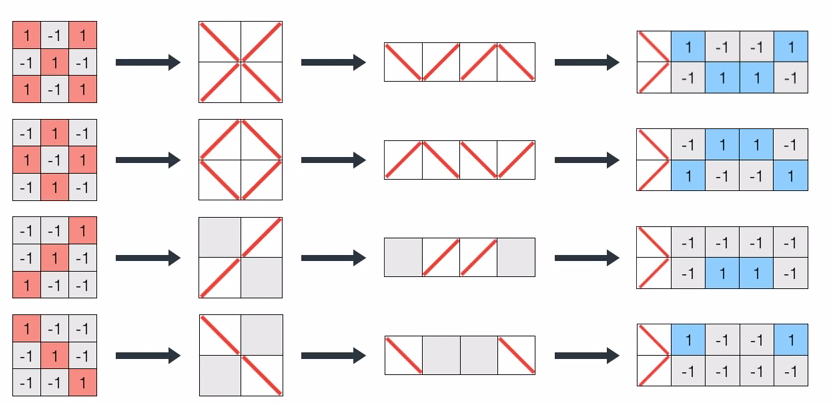
\includegraphics[width=0.6\linewidth,keepaspectratio]{cnn31}
% \end{center}
% \end{frame}

% %%%%%%%%%%%%%%%%%%%%%%%%%%%%%%%%%%%%%%%%%%%%%%%%%%%
% \begin{frame}[fragile] \frametitle{Toy Example: Image Recognition Classifier}
% \begin{itemize}
% \item  With these values we can create the filters
% \item Each filter is for a specific output
% \end{itemize}
% \begin{center}
% 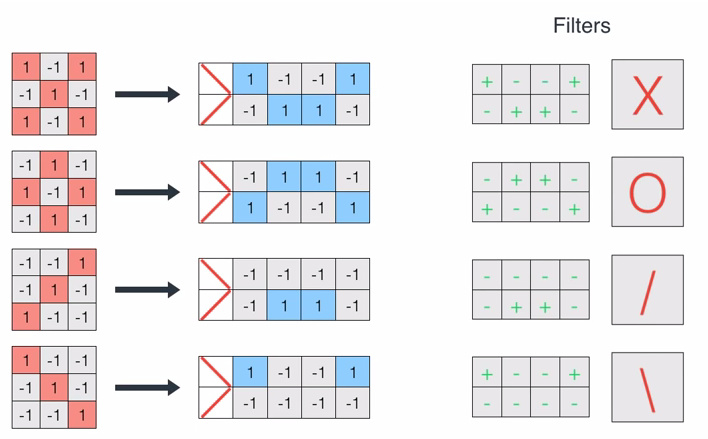
\includegraphics[width=0.8\linewidth,keepaspectratio]{cnn32}
% \end{center}
% \end{frame}

% %%%%%%%%%%%%%%%%%%%%%%%%%%%%%%%%%%%%%%%%%%%%%%%%%%%
% \begin{frame}[fragile] \frametitle{Toy Example: Image Recognition Classifier}
% \begin{itemize}
% \item Overlap  all filters one by one and get the score.
% \item Scores are 8, -8, 4, 4.
% \item Max is the winner
% \item So 3x3 image on the left is X
% \end{itemize}
% \begin{center}
% 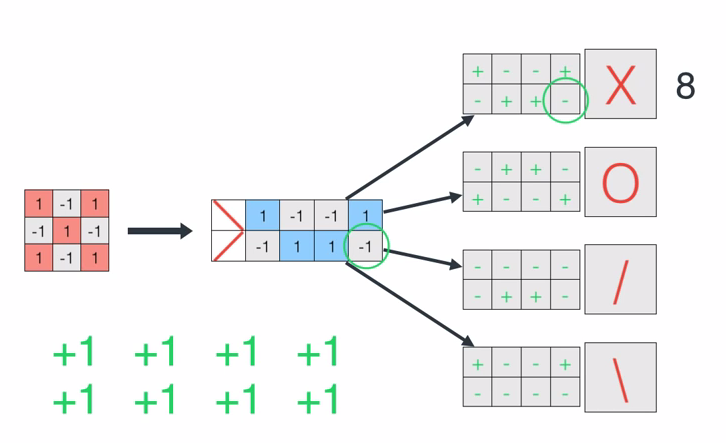
\includegraphics[width=0.8\linewidth,keepaspectratio]{cnn33}
% \end{center}
% \end{frame}

% %%%%%%%%%%%%%%%%%%%%%%%%%%%%%%%%%%%%%%%%%%%%%%%%%%%
% \begin{frame}[fragile] \frametitle{Toy Example: Image Recognition Classifier}
% For ``O''
% \begin{center}
% \includegraphics[width=\linewidth,keepaspectratio]{cnn34}
% \end{center}
% \end{frame}

% %%%%%%%%%%%%%%%%%%%%%%%%%%%%%%%%%%%%%%%%%%%%%%%%%%%
% \begin{frame}[fragile] \frametitle{Toy Example: Image Recognition Classifier}
 % We had pixeletted 4 images, which we want to classify. For each we do following procedure

% \begin{itemize}
% \item Apply two filters (one for forward and one for backward slash)
% \item They go total 4+4 places.
% \item Pooling finds  b-slash or f-slash at places, based on the score and threshold
% \item Now the original image gets converted to 2x4 matrix
% \item We try all 4 plus-minus filters on each and find scores
% \item Logic using Max on filter scores, declares the class
% \end{itemize}
% \end{frame}


% %%%%%%%%%%%%%%%%%%%%%%%%%%%%%%%%%%%%%%%%%%%%%%%%%%%
% \begin{frame}[fragile] \frametitle{Toy Example: Image Recognition Classifier}
% Summary for X
% \begin{center}
% \includegraphics[width=\linewidth,keepaspectratio]{cnn36}
% \end{center}
% \end{frame}

% %%%%%%%%%%%%%%%%%%%%%%%%%%%%%%%%%%%%%%%%%%%%%%%%%%%
% \begin{frame}[fragile] \frametitle{Toy Example: Image Recognition Classifier}
% Practically:
% \begin{itemize}
% \item Starts with random filter values.
% \item Predicts, finds errors
% \item Gradient Descent to min error
% \end{itemize}
% \begin{center}
% \includegraphics[width=\linewidth,keepaspectratio]{cnn37}
% \end{center}
% \end{frame}


% %%%%%%%%%%%%%%%%%%%%%%%%%%%%%%%%%%%%%%%%%%%%%%%%%%%
% \begin{frame}
  % \begin{center}
    % {\Large CNN : Intuition with a case study}
  % \end{center}
% \end{frame}


% %%%%%%%%%%%%%%%%%%%%%%%%%%%%%%%%%%%%%%%%%%%%%%%%%%%
% \begin{frame}[fragile] \frametitle{Intuition with a case study}
% Input:

% \begin{itemize}
% \item An Image is a matrix of pixel values
% \item Channel is a conventional term used to refer to a certain component of an image. 
% \item An image from a standard digital camera will have three channels : red, green and blue
% \item You can imagine those as three 2d-matrices stacked over each other (one for each color), each having pixel values in the range 0 to 255.
% \end{itemize}
% \end{frame}

% %%%%%%%%%%%%%%%%%%%%%%%%%%%%%%%%%%%%%%%%%%%%%%%%%%%
% \begin{frame}[fragile] \frametitle{Intuition with a case study}

% Input:
% \begin{itemize}
% \item A grayscale image, on the other hand, has just one channel.
% \item For the purpose of this post, we will only consider grayscale images, so we will have a single 2d matrix representing an image. 
% \item The value of each pixel in the matrix will range from 0 to 255 : zero indicating black and 255 indicating white.
% \end{itemize}
% \end{frame}

% %%%%%%%%%%%%%%%%%%%%%%%%%%%%%%%%%%%%%%%%%%%%%%%%%%%
% \begin{frame}[fragile] \frametitle{Intuition with a case study}

% The Convolution Step:
% \begin{itemize}
% \item ConvNets derive their name from the ``convolution'' operator. 
% \item The primary purpose of Convolution in case of a ConvNet is to extract features from the input image. 
% \item Convolution preserves the spatial relationship between pixels by learning image features using small squares of input data. 
% \end{itemize}
% \end{frame}

% %%%%%%%%%%%%%%%%%%%%%%%%%%%%%%%%%%%%%%%%%%%%%%%%%%%
% \begin{frame}[fragile] \frametitle{Intuition with a case study}

% The Convolution Step:
% \begin{itemize}
% \item Consider a 5 x 5 image whose pixel values are only 0 and 1
% \item Note that for a grayscale image, pixel values range from 0 to 255, the green matrix below is a special case where pixel values are only 0 and 1
% \item Also, consider another 3 x 3 matrix as shown below:
% \end{itemize}
% \begin{center}
% \includegraphics[width=0.3\linewidth,keepaspectratio]{cnn3} \quad
% \includegraphics[width=0.2\linewidth,keepaspectratio]{cnn4}
% \end{center}
% \end{frame}

% %%%%%%%%%%%%%%%%%%%%%%%%%%%%%%%%%%%%%%%%%%%%%%%%%%%
% \begin{frame}[fragile] \frametitle{Intuition with a case study}

% The Convolution Step:
% \begin{itemize}
% \item  the Convolution of the 5 x 5 image and the 3 x 3 matrix can be computed 
% \item Slide the orange matrix over our original image (green) by 1 pixel (also called 'stride')
% \end{itemize}
% \begin{center}
% \includegraphics[width=0.6\linewidth,keepaspectratio]{cnn5}
% \end{center}
% \end{frame}


% %%%%%%%%%%%%%%%%%%%%%%%%%%%%%%%%%%%%%%%%%%%%%%%%%%%
% \begin{frame}[fragile] \frametitle{Intuition with a case study}

% The Convolution Step:
% \begin{itemize}
% \item  For every position, we compute element wise multiplication (between the two matrices) and add the multiplication outputs to get the final integer which forms a single element of the output matrix (pink).
% \item Note that the 3x3 matrix ``sees'' only a part of the input image in each stride.
% \end{itemize}
% \begin{center}
% \includegraphics[width=0.6\linewidth,keepaspectratio]{cnn5}
% \end{center}
% \end{frame}

% %%%%%%%%%%%%%%%%%%%%%%%%%%%%%%%%%%%%%%%%%%%%%%%%%%%
% \begin{frame}[fragile] \frametitle{Intuition with a case study}

% The Convolution Step:
% \begin{itemize}
% \item  The 3x3 matrix is called a 'filter' or 'kernel' or 'feature detector' and the matrix formed by sliding the filter over the image and computing the dot product is called the 'Convolved Feature' or 'Activation Map' or the 'Feature Map'. 
% \item It is important to note that filters acts as feature detectors from the original input image.
% \item different values of the filter matrix will produce different Feature Maps for the same input image.
% \end{itemize}

% \end{frame}


% %%%%%%%%%%%%%%%%%%%%%%%%%%%%%%%%%%%%%%%%%%%%%%%%%%%
% \begin{frame}[fragile] \frametitle{Intuition with a case study}
% the effects of convolution of the above image with different filters.
% \begin{center}
% \includegraphics[width=0.4\linewidth,keepaspectratio]{cnn6}
% \end{center}

% \end{frame}

% %%%%%%%%%%%%%%%%%%%%%%%%%%%%%%%%%%%%%%%%%%%%%%%%%%%
% \begin{frame}[fragile] \frametitle{Intuition with a case study}

% The Convolution Step:
% \begin{itemize}
% \item  In practice, a CNN learns the values of these filters on its own during the training process
% \item The more number of filters we have, the more image features get extracted and the better our network becomes at recognizing patterns in unseen images.
% \end{itemize}

% \end{frame}

% %%%%%%%%%%%%%%%%%%%%%%%%%%%%%%%%%%%%%%%%%%%%%%%%%%%
% \begin{frame}[fragile] \frametitle{Intuition with a case study}

% The size of the Feature Map (Convolved Feature) is controlled by three parameters
% \begin{itemize}
% \item  Depth
% \item Stride
% \item Padding
% \end{itemize}

% \end{frame}

% %%%%%%%%%%%%%%%%%%%%%%%%%%%%%%%%%%%%%%%%%%%%%%%%%%%
% \begin{frame}[fragile] \frametitle{Intuition with a case study}

% Depth:
% \begin{itemize}
% \item  Depth corresponds to the number of filters 
% \item performing convolution of the original boat image using three distinct filters, thus producing three different feature maps as shown. 
% \item You can think of these three feature maps as stacked 2d matrices, so, the `depth' of the feature map would be three.
% \end{itemize}
% \begin{center}
% \includegraphics[width=0.6\linewidth,keepaspectratio]{cnn7}
% \end{center}
% \end{frame}


% %%%%%%%%%%%%%%%%%%%%%%%%%%%%%%%%%%%%%%%%%%%%%%%%%%%
% \begin{frame}[fragile] \frametitle{Intuition with a case study}

% Stride:
% \begin{itemize}
% \item  Stride is the number of pixels by which we slide our filter matrix over the input matrix. 
% \item When the stride is 1 then we move the filters one pixel at a time. 
% \item When the stride is 2, then the filters jump 2 pixels at a time as we slide them around. 
% \item Having a larger stride will produce smaller feature maps.
% \end{itemize}

% \end{frame}

% %%%%%%%%%%%%%%%%%%%%%%%%%%%%%%%%%%%%%%%%%%%%%%%%%%%
% \begin{frame}[fragile] \frametitle{Intuition with a case study}

% Padding:
% \begin{itemize}
% \item  Sometimes, it is convenient to pad the input matrix with zeros around the border, so that we can apply the filter to bordering elements of our input image matrix. 
% \item A nice feature of zero padding is that it allows us to control the size of the feature maps. 
% \item Adding zero-padding is also called wide convolution, and not using zero-padding would be a narrow convolution. 
% \end{itemize}

% \end{frame}


% %%%%%%%%%%%%%%%%%%%%%%%%%%%%%%%%%%%%%%%%%%%%%%%%%%%
% \begin{frame}[fragile] \frametitle{Intuition with a case study}

% Introducing Non Linearity (ReLU):
% \begin{itemize}
% \item  ReLU stands for Rectified Linear Unit and is a non-linear operation.
% \item Its output is given by
% \end{itemize}
% \begin{center}
% \includegraphics[width=\linewidth,keepaspectratio]{cnn8}
% \end{center}
% \end{frame}


% %%%%%%%%%%%%%%%%%%%%%%%%%%%%%%%%%%%%%%%%%%%%%%%%%%%
% \begin{frame}[fragile] \frametitle{Intuition with a case study}

% Introducing Non Linearity (ReLU):
% \begin{itemize}
% \item  ReLU is an element wise operation (applied per pixel) and replaces all negative pixel values in the feature map by zero. 
% \item Convolution is a linear operation : element wise matrix multiplication and addition, so we account for non-linearity by introducing a non-linear function like ReLU
% \end{itemize}

% \end{frame}

% %%%%%%%%%%%%%%%%%%%%%%%%%%%%%%%%%%%%%%%%%%%%%%%%%%%
% \begin{frame}[fragile] \frametitle{Intuition with a case study}

% Introducing Non Linearity (ReLU):
% \begin{itemize}
% \item   shows the ReLU operation applied to one of the feature maps 
% \item The output feature map here is also referred to as the `Rectified' feature map.
% \end{itemize}
% \begin{center}
% \includegraphics[width=0.6\linewidth,keepaspectratio]{cnn9}
% \end{center}
% Other non linear functions such as tanh or sigmoid can also be used instead of ReLU, but ReLU has been found to perform better in most situations.
% \end{frame}

% %%%%%%%%%%%%%%%%%%%%%%%%%%%%%%%%%%%%%%%%%%%%%%%%%%%
% \begin{frame}[fragile] \frametitle{Intuition with a case study}

% The Pooling Step:
% \begin{itemize}
% \item  Pooling (also called subsampling or downsampling) reduces the dimensionality of each feature map but retains the most important information. 
% \item Pooling can be of different types: Max, Average, Sum etc.
% \end{itemize}

% \end{frame}

% %%%%%%%%%%%%%%%%%%%%%%%%%%%%%%%%%%%%%%%%%%%%%%%%%%%
% \begin{frame}[fragile] \frametitle{Intuition with a case study}

% The Pooling Step:
% \begin{itemize}
% \item  In case of Max Pooling, we define a spatial neighborhood (for example, a 2x2 window) and take the largest element from the rectified feature map within that window.
% \item Instead of taking the largest element we could also take the average (Average Pooling) or sum of all elements in that window. 
% \item In practice, Max Pooling has been shown to work better.
% \end{itemize}

% \end{frame}


% %%%%%%%%%%%%%%%%%%%%%%%%%%%%%%%%%%%%%%%%%%%%%%%%%%%
% \begin{frame}[fragile] \frametitle{Intuition with a case study}

% The Pooling Step:
% \begin{center}
% \includegraphics[width=0.6\linewidth,keepaspectratio]{cnn10}
% \end{center}
% We slide our 2 x 2 window by 2 cells (also called `stride') and take the maximum value in each region. As shown, this reduces the dimensionality of our feature map.
% \end{frame}

% %%%%%%%%%%%%%%%%%%%%%%%%%%%%%%%%%%%%%%%%%%%%%%%%%%%
% \begin{frame}[fragile] \frametitle{Intuition with a case study}
% In the network shown, pooling operation is applied separately to each feature map (notice that, due to this, we get three output maps from three input maps).
% \begin{center}
% \includegraphics[width=0.8\linewidth,keepaspectratio]{cnn11}
% \end{center}

% \end{frame}


% %%%%%%%%%%%%%%%%%%%%%%%%%%%%%%%%%%%%%%%%%%%%%%%%%%%
% \begin{frame}[fragile] \frametitle{Intuition with a case study}
% Shows the effect of Pooling on the Rectified Feature Map we received after the ReLU operation
% \begin{center}
% \includegraphics[width=0.8\linewidth,keepaspectratio]{cnn12}
% \end{center}

% \end{frame}

% %%%%%%%%%%%%%%%%%%%%%%%%%%%%%%%%%%%%%%%%%%%%%%%%%%%
% \begin{frame}[fragile] \frametitle{Intuition with a case study}

% The Pooling Step:
% \begin{itemize}
% \item makes the input representations (feature dimension) smaller and more manageable
% \item reduces the number of parameters and computations in the network, therefore, controlling overfitting
% \item makes the network invariant to small transformations, distortions and translations in the input image (a small distortion in input will not change the output of Pooling : since we take the maximum / average value in a local neighborhood).
% \item helps us arrive at an almost scale invariant representation of our image (the exact term is ``equivariant''). This is very powerful since we can detect objects in an image no matter where they are located
% \end{itemize}

% \end{frame}

% %%%%%%%%%%%%%%%%%%%%%%%%%%%%%%%%%%%%%%%%%%%%%%%%%%%
% \begin{frame}[fragile] \frametitle{Intuition with a case study}

% Story so far:
% \begin{center}
% \includegraphics[width=\linewidth,keepaspectratio]{cnn13}
% \end{center}


% \begin{itemize}
% \item So far we have seen how Convolution, ReLU and Pooling work.
% \item we have two sets of Convolution, ReLU \& Pooling layers : the 2nd Convolution layer performs convolution on the output of the first Pooling Layer using six filters to produce a total of six feature maps. 
% \end{itemize}

% \end{frame}


% %%%%%%%%%%%%%%%%%%%%%%%%%%%%%%%%%%%%%%%%%%%%%%%%%%%
% \begin{frame}[fragile] \frametitle{Intuition with a case study}

% Story so far:
% \begin{center}
% \includegraphics[width=\linewidth,keepaspectratio]{cnn13}
% \end{center}


% \begin{itemize}
% \item ReLU is then applied individually on all of these six feature maps. 
% \item We then perform Max Pooling operation separately on each of the six rectified feature maps.
% \end{itemize}

% \end{frame}



% %%%%%%%%%%%%%%%%%%%%%%%%%%%%%%%%%%%%%%%%%%%%%%%%%%%
% \begin{frame}[fragile] \frametitle{Intuition with a case study}
% Story so far:
% \begin{itemize}
% \item Together these layers extract the useful features from the images, introduce non-linearity in our network and reduce feature dimension while aiming to make the features somewhat equivariant to scale and translation
% \item The output of the 2nd Pooling Layer acts as an input to the Fully Connected Layer
% \end{itemize}
% \end{frame}


% %%%%%%%%%%%%%%%%%%%%%%%%%%%%%%%%%%%%%%%%%%%%%%%%%%%
% \begin{frame}[fragile] \frametitle{Intuition with a case study}
% Fully Connected Layer:
% \begin{itemize}
% \item The Fully Connected layer is a traditional Multi Layer Perceptron that uses a softmax activation function in the output layer.
% \item The term “Fully Connected” implies that every neuron in the previous layer is connected to every neuron on the next layer.
% \item The output from the convolutional and pooling layers represent high-level features of the input image. 
% \item The purpose of the Fully Connected layer is to use these features for classifying the input image into various classes based on the training dataset.
% \end{itemize}
% \end{frame}


% %%%%%%%%%%%%%%%%%%%%%%%%%%%%%%%%%%%%%%%%%%%%%%%%%%%
% \begin{frame}[fragile] \frametitle{Intuition with a case study}

% Fully Connected Layer:
% \begin{itemize}
% \item  For example, the image classification task we set out to perform has four possible outputs
% \item Apart from classification, adding a fully-connected layer is also a (usually) cheap way of learning non-linear combinations of these features. 
% \item Most of the features from convolutional and pooling layers may be good for the classification task, but combinations of those features might be even better
% \end{itemize}
% \begin{center}
% \includegraphics[width=0.7\linewidth,keepaspectratio]{cnn14}
% \end{center}
% \end{frame}

% %%%%%%%%%%%%%%%%%%%%%%%%%%%%%%%%%%%%%%%%%%%%%%%%%%%
% \begin{frame}[fragile] \frametitle{Intuition with a case study}

% Fully Connected Layer:
% \begin{itemize}
% \item  The sum of output probabilities from the Fully Connected Layer is 1.
% \item  This is ensured by using the Softmax as the activation function in the output layer of the Fully Connected Layer. 
% \item The Softmax function takes a vector of arbitrary real-valued scores and squashes it to a vector of values between zero and one that sum to one.
% \end{itemize}
% \end{frame}

% %%%%%%%%%%%%%%%%%%%%%%%%%%%%%%%%%%%%%%%%%%%%%%%%%%%
% \begin{frame}[fragile] \frametitle{Intuition with a case study}

% Putting it all together - Training using Backpropagation:
% \begin{itemize}
% \item  the Convolution + Pooling layers act as Feature Extractors from the input image while Fully Connected layer acts as a classifier.
% \item since the input image is a boat, the target probability is 1 for Boat class and 0 for other three classes
% \end{itemize}
% \end{frame}

% %%%%%%%%%%%%%%%%%%%%%%%%%%%%%%%%%%%%%%%%%%%%%%%%%%%
% \begin{frame}[fragile] \frametitle{Intuition with a case study}

% Putting it all together - Training using Backpropagation:
% \begin{itemize}
% \item  Input Image = Boat
% \item  Target Vector = $[0, 0, 1, 0]$
% \end{itemize}
% \begin{center}
% \includegraphics[width=0.7\linewidth,keepaspectratio]{cnn15}
% \end{center}
% \end{frame}

% %%%%%%%%%%%%%%%%%%%%%%%%%%%%%%%%%%%%%%%%%%%%%%%%%%%
% \begin{frame}[fragile] \frametitle{Intuition with a case study}

% Putting it all together - Training using Backpropagation:
% \begin{itemize}
% \item  Step1: We initialize all filters and parameters / weights with random values
% \item Step2: The network takes a training image as input, goes through the forward propagation step (convolution, ReLU and pooling operations along with forward propagation in the Fully Connected layer) 
% \end{itemize}
% \begin{center}
% \includegraphics[width=0.7\linewidth,keepaspectratio]{cnn15}
% \end{center}
% \end{frame}

% %%%%%%%%%%%%%%%%%%%%%%%%%%%%%%%%%%%%%%%%%%%%%%%%%%%
% \begin{frame}[fragile] \frametitle{Intuition with a case study}

% Putting it all together - Training using Backpropagation:
% \begin{itemize}
% \item  Finds the output probabilities for each class.
% \item  Lets say the output probabilities for the boat image above are [0.2, 0.4, 0.1, 0.3]
% \item  Since weights are randomly assigned for the first training example, output probabilities are also random.
 % Connected layer) 
% \end{itemize}
% \begin{center}
% \includegraphics[width=0.7\linewidth,keepaspectratio]{cnn15}
% \end{center}
% \end{frame}

% %%%%%%%%%%%%%%%%%%%%%%%%%%%%%%%%%%%%%%%%%%%%%%%%%%%
% \begin{frame}[fragile] \frametitle{Intuition with a case study}

% Putting it all together - Training using Backpropagation:
% \begin{itemize}
% \item  Step3: Calculate the total error at the output layer (summation over all 4 classes) 
% \item $Total Error =  1/2 \sum (TargetProbability - OutputProbability)^2$
% \end{itemize}
% \begin{center}
% \includegraphics[width=0.7\linewidth,keepaspectratio]{cnn15}
% \end{center}
% \end{frame}

% %%%%%%%%%%%%%%%%%%%%%%%%%%%%%%%%%%%%%%%%%%%%%%%%%%%
% \begin{frame}[fragile] \frametitle{Intuition with a case study}

% Putting it all together - Training using Backpropagation:
% \begin{itemize}
% \item  Step4: Use Backpropagation to calculate the gradients of the error with respect to all weights in the network and use gradient descent to update all filter values / weights and parameter values to minimize the output error. 
% \item The weights are adjusted in proportion to their contribution to the total error.
% \item When the same image is input again, output probabilities might now be [0.1, 0.1, 0.7, 0.1], which is closer to the target vector [0, 0, 1, 0].
% \end{itemize}

% \end{frame}

% %%%%%%%%%%%%%%%%%%%%%%%%%%%%%%%%%%%%%%%%%%%%%%%%%%%
% \begin{frame}[fragile] \frametitle{Intuition with a case study}

% Putting it all together - Training using Backpropagation:
% \begin{itemize}
% \item  This means that the network has learnt to classify this particular image correctly by adjusting its weights / filters such that the output error is reduced.
% \item Parameters like number of filters, filter sizes, architecture of the network etc. have all been fixed before Step 1 and do not change during training process - only the values of the filter matrix and connection weights get updated.
% \end{itemize}

% \end{frame}

% %%%%%%%%%%%%%%%%%%%%%%%%%%%%%%%%%%%%%%%%%%%%%%%%%%%
% \begin{frame}[fragile] \frametitle{Intuition with a case study}

% Putting it all together - Training using Backpropagation:
% \begin{itemize}
% \item  Step5: Repeat steps 2-4 with all images in the training set.
% \item The above steps train the ConvNet - this essentially means that all the weights and parameters of the ConvNet have now been optimized to correctly classify images from the training set.
% \end{itemize}
% \begin{center}
% \includegraphics[width=0.7\linewidth,keepaspectratio]{cnn15}
% \end{center}
% \end{frame}


% %%%%%%%%%%%%%%%%%%%%%%%%%%%%%%%%%%%%%%%%%%%%%%%%%%%
% \begin{frame}[fragile] \frametitle{Intuition with a case study}

% Putting it all together - Training using Backpropagation:
% \begin{itemize}
% \item  When a new (unseen) image is input into the ConvNet, the network would go through the forward propagation step and output a probability for each class (for a new image, the output probabilities are calculated using the weights which have been optimized to correctly classify all the previous training examples). 
% \item If our training set is large enough, the network will (hopefully) generalize well to new images and classify them into correct categories.
% \end{itemize}
% \end{frame}







%%%%%%%%%%%%%%%%%%%%%%%%%%%%%%%%%%%%%%%%%%%%%%%%%%%
\begin{frame}[fragile] \frametitle{CNN Architecture (Recap)}

\begin{itemize}
\item The Convolutional layer consists of a set of filters.
\item Each filter covers a spatially small portion of the input data.
\item Each filter is convolved across the dimensions of the input data, producing a multidimensional feature map.
\item As we convolve the filter, we are computing the dot product between the parameters of the filter and the input.
\end{itemize}
\end{frame}


%%%%%%%%%%%%%%%%%%%%%%%%%%%%%%%%%%%%%%%%%%%%%%%%%%%
\begin{frame}[fragile] \frametitle{CNN Architecture (Recap)}

\begin{itemize}
\item Intuition: the network will learn filters that activate when they see some specific type of feature at some spatial position in the input.
\begin{itemize}
\item Stacking multiple layers of feature extractors
\item Low-level layers extract local features.
\item High-level layers extract learn global patterns.
\end{itemize}
\item The key architectural characteristics of the convolutional layer is local connectivity and shared weights.
\end{itemize}
\end{frame}


%%%%%%%%%%%%%%%%%%%%%%%%%%%%%%%%%%%%%%%%%%%%%%%%%%%
\begin{frame}[fragile] \frametitle{CNN Architecture (Recap)}
\begin{itemize}
\item A CNN is a list of layers that transform the input data into an output class/prediction.
\item There are a few distinct types of layers:
\begin{itemize}
\item Convolutional layer
\item Non-linear layer
\item Pooling layer
\end{itemize}
\end{itemize}
\end{frame}


%%%
%%%
%%%%%%%%%%%%%%%%%%%%%%%%%%%%%%%%%%%%%%%%%%%%%%%%%%%%%%
%%%\begin{frame}[fragile] \frametitle{CNN Convolutional Layer: Local Connectivity}
%%%
%%%\adjustbox{valign=t}{
%%%\begin{minipage}{0.45\linewidth}
%%%\begin{itemize}
%%%\item Neurons in layer $m$ are only connected to 3 adjacent neurons in the $m-1$ layer.
%%%\item Similarly for $m+1$. 
%%%\item Each neuron is unresponsive to variations outside. 
%%%\item Receptive field: small neuron collections which process portions of the input data
%%%\item Strongest response to a spatially local input pattern.
%%%\end{itemize}
%%%\end{minipage}
%%%}
%%%\hfill
%%%\adjustbox{valign=t}{
%%%\begin{minipage}{0.45\linewidth}
%%%\begin{center}
%%%\includegraphics[width=\linewidth,keepaspectratio]{cnnlocal}
%%%\end{center}
%%%\end{minipage}
%%%}
%%%
%%%\end{frame}
%%%
%%%
%%%%%%%%%%%%%%%%%%%%%%%%%%%%%%%%%%%%%%%%%%%%%%%%%%%%%%
%%%\begin{frame}[fragile] \frametitle{CNN Convolutional Layer: Shared Weights}
%%%
%%%\adjustbox{valign=t}{
%%%\begin{minipage}{0.45\linewidth}
%%%\begin{itemize}
%%%\item Weights of the same color are shared. 
%%%\item Gradient descent can still be used
%%%\item Replicating neurons in this way allows for features to be detected regardless of their position in the input. 
%%%\end{itemize}
%%%\end{minipage}
%%%}
%%%\hfill
%%%\adjustbox{valign=t}{
%%%\begin{minipage}{0.45\linewidth}
%%%3 hidden neurons belonging to the same feature map (the layer right above the input layer). 
%%%\begin{center}
%%%\includegraphics[width=0.8\linewidth,keepaspectratio]{cnnwts}
%%%\end{center}
%%%Weight sharing increases learning efficiency by reducing the number of free parameters being learnt.
%%%\end{minipage}
%%%}
%%%
%%%\end{frame}
%%%
%%%
%%%
%%%%%%%%%%%%%%%%%%%%%%%%%%%%%%%%%%%%%%%%%%%%%%%%%%%%%%
%%%\begin{frame}[fragile] \frametitle{CNN Architecture: Non-linear Layer}
%%%
%%%\begin{itemize}
%%%\item Intuition: Increase the nonlinearity of the entire architecture without affecting the receptive fields of the convolution layer
%%%\item A layer of neurons that applies the non-linear activation function, such as,
%%%\begin{itemize}
%%%\item $f(x) = max(0,x)$
%%%\item $f(x) = tanh(x)$
%%%\item $f(x) = | tanh(x) |$
%%%\item $f(x) = (1 + e^{-x})^{-1}$
%%%\end{itemize}
%%%\end{itemize}
%%%\end{frame}
%%%
%%%%%%%%%%%%%%%%%%%%%%%%%%%%%%%%%%%%%%%%%%%%%%%%%%%%%%
%%%\begin{frame}[fragile] \frametitle{CNN Architecture: Pooling Layer}
%%%
%%%\begin{itemize}
%%%\item Intuition: to progressively reduce the spatial size of the representation to reduce the amount of parameters and computation in the network, and hence to also control overfitting
%%%\item Pooling partitions the input image into a set of non-overlapping rectangles and, for each such sub-region, outputs the maximum value of the features in that region.
%%%\end{itemize}
%%%\begin{center}
%%%\includegraphics[width=0.8\linewidth,keepaspectratio]{cnnpool}
%%%\end{center}
%%%\end{frame}
%%%


%%%%%%%%%%%%%%%%%%%%%%%%%%%%%%%%%%%%%%%%%%%%%%%%%%%%
%\begin{frame}[fragile] \frametitle{Convolutional Neural Networks}
%Convolution layers are a variant on the dense linear layers. They simultaneously address
%several issues commonly seen in computer vision applications: 
%\begin{itemize}
%\item To utilize the known geometry of the data (color channels
%and locality)
%\item Larger images require an enormous number of weights for even modestly
%sized hidden layers. Using $96x96$ pixel images and a single hidden layer with
%$1024$ nodes, requires just under ten million individual weights!
%\item To have a method
%that is insensitive to small shifts in the individual pixels.
%\end{itemize}
%Apart from 2D-convolutions in image processing, 1D, 3D
%and higher dimensions convolutions are possible.
%\end{frame}
%
%%%%%%%%%%%%%%%%%%%%%%%%%%%%%%%%%%%%%%%%%%%%%%%%%%%%
%\begin{frame}[fragile] \frametitle{}
%Convolution layers are like a dense/linear layer, with two constraints applied to the weights and biases.
%\begin{itemize}
%\item Sparsity with local receptive field: the weight and biases for a given neuron
%are only non-zero over a small, local region of the input image.
%\item Shared weights: the non-zero weights and biases are the same across all of the
%neurons, up to a shifting over the image.
%\end{itemize}
%\end{frame}
%
%
%
%
%%%%%%%%%%%%%%%%%%%%%%%%%%%%%%%%%%%%%%%%%%%%%%%%%%%%
%\begin{frame}[fragile] \frametitle{First position}
%
%\begin{center}
%\includegraphics[width=0.8\linewidth,keepaspectratio]{tikz44.png}
%\end{center}
%
%\end{frame}
%
%%%%%%%%%%%%%%%%%%%%%%%%%%%%%%%%%%%%%%%%%%%%%%%%%%%%
%\begin{frame}[fragile] \frametitle{Second position}
%
%\begin{center}
%\includegraphics[width=0.8\linewidth,keepaspectratio]{tikz45.png}
%\end{center}
%
%\end{frame}
%
%%%%%%%%%%%%%%%%%%%%%%%%%%%%%%%%%%%%%%%%%%%%%%%%%%%%
%\begin{frame}[fragile] \frametitle{Filters}
%
%\begin{itemize}
%\item  A convolutional layer is made up of some predetermined
%number of filters.
%are only non-zero over a small, local region of the input image.
%\item That is, we have multiple set of local
%weights that are applied over small chunks of the image.
%\item These allow us to capture different components that may
%all be useful for the classification task at hand.
%\end{itemize}
% 
%
%\end{frame}
%
%%%%%%%%%%%%%%%%%%%%%%%%%%%%%%%%%%%%%%%%%%%%%%%%%%%%
%\begin{frame}[fragile] \frametitle{Filters: History}
%
%
%The idea of using a filter on images is not a new idea to
%neural networks; the difference here is the filters are
%adaptively learned from data.
%
%For example, take the following fixed kernel weights:
%\begin{align*}
%\left(\begin{array}{cc} 1 & 0 \\ 0 & -1 \end{array} \right)
%\end{align*}
%What happens when we apply this over an image?
%
%\end{frame}
%
%%%%%%%%%%%%%%%%%%%%%%%%%%%%%%%%%%%%%%%%%%%%%%%%%%%%
%\begin{frame}[fragile] \frametitle{}
%
%\begin{center}
%\includegraphics[width=0.8\linewidth,keepaspectratio]{both.jpg}
%\end{center}
%
%\end{frame}
%
%%%%%%%%%%%%%%%%%%%%%%%%%%%%%%%%%%%%%%%%%%%%%%%%%%%%
%\begin{frame}[fragile] \frametitle{}
%
%\begin{center}
%\includegraphics[width=0.8\linewidth,keepaspectratio]{gabor.jpg}
%\end{center}
%
%\end{frame}
%
%%%%%%%%%%%%%%%%%%%%%%%%%%%%%%%%%%%%%%%%%%%%%%%%%%%%
%\begin{frame}[fragile] \frametitle{}
%
%A convolutional layer with $3$ filters:
%
%\begin{center}
%\includegraphics[width=0.8\linewidth,keepaspectratio]{tikz46.png}
%\end{center}
%
%\end{frame}
%
%%%%%%%%%%%%%%%%%%%%%%%%%%%%%%%%%%%%%%%%%%%%%%%%%%%%
%\begin{frame}[fragile] \frametitle{Zero padding}
%
%You may have noticed that the grid of pixels of the output image
%will have fewer rows and columns than the input image.
%In some cases this is okay, but it is often advantageous to
%preserve the size of the grid (there are several reasons that we
%want to grid size to be divisible by $2^n$ for some reasonably large
%$n$). To do so, we can add extra rows and columns of zeros
%(zero padding) to the input before applying the
%
%\end{frame}
%
%%%%%%%%%%%%%%%%%%%%%%%%%%%%%%%%%%%%%%%%%%%%%%%%%%%%
%\begin{frame}[fragile] \frametitle{Kernel and stride}
%
%The architecture of a (2D) convolution layer is primarily
%determined by four numbers:
%\begin{itemize}
%\item the number of filters, F
%\item the height of the kernel, $k_h$
%\item the width of the kernel, $k_w$
%\item the stride, $k_s$
%\end{itemize}
%The stride tells us how far the local set of weights is
%shifted before being applied. We'll mostly use a stride
%of $1$, but just note that other values are possible.
%
%\end{frame}
%
%%%%%%%%%%%%%%%%%%%%%%%%%%%%%%%%%%%%%%%%%%%%%%%%%%%%
%\begin{frame}[fragile] \frametitle{}
%
%A 5x5 kernel:
%
%\begin{center}
%\includegraphics[width=0.8\linewidth,keepaspectratio]{tikz44.png}
%\end{center}
%
%\end{frame}
%
%%%%%%%%%%%%%%%%%%%%%%%%%%%%%%%%%%%%%%%%%%%%%%%%%%%%
%\begin{frame}[fragile] \frametitle{}
%
%A stride of $1$:
%
%\begin{center}
%\includegraphics[width=0.8\linewidth,keepaspectratio]{tikz45.png}
%\end{center}
%
%\end{frame}
%
%%%%%%%%%%%%%%%%%%%%%%%%%%%%%%%%%%%%%%%%%%%%%%%%%%%%
%\begin{frame}[fragile] \frametitle{}
%
%A nice demo of applying convolution over a grid using alternative
%strides and zero padding:
%
%\begin{center}
%\url{http://cs231n.github.io/assets/conv-demo/index.html}
%\end{center}
%
%\end{frame}
%
%%%%%%%%%%%%%%%%%%%%%%%%%%%%%%%%%%%%%%%%%%%%%%%%%%%%
%\begin{frame}[fragile] \frametitle{Tensors}
%
%A convolution can also be described in purely algebraic
%terms. We are defining a map from a three dimensional space
%to a three dimensional space:
%\begin{align*}
%F^1 \times W^1 \times H^1 \rightarrow F^2 \times W^2 \times H^2
%\end{align*}
%Where $F$ is the number of filters, $W$ the width of the image,
%and $H$ the height of the image. You can now see why tensors are
%considered a generalization of a matrix operations, and why they
%are so important in learning neural network models.
%
%\pause The value $F^1$ is equal to one for the MNIST dataset, but
%for CIFAR-10 we would set it to $3$ to deal with the $3$ color
%channels.
%
%\end{frame}
%
%%%%%%%%%%%%%%%%%%%%%%%%%%%%%%%%%%%%%%%%%%%%%%%%%%%%
%\begin{frame}[fragile] \frametitle{Pooling layers}
%
%Convolutional neural networks have another type of layer that can
%also be described by applying a function locally to small section
%of the image. These layers are called pooling layers; they differ
%from convolution layers because:
%\begin{itemize}
%\item they have no learned weights
%\item may not be linear functions of their inputs
%\item are applied separately to each kernel
%\item the stride is usually equal to the size of the kernel; that is,
%the regions are non-overlapping
%\end{itemize}
%The most common type of pooling (by far) is called max-pooling, with
%a 2x2 kernel and stride of $2$.
%This halves the extent of each dimension (reduces the
%number of data points by a factor of $4$ for 2D images) and can greatly
%decrease the learning time and improve over-fitting of the data.
%
%\end{frame}
%
%%%%%%%%%%%%%%%%%%%%%%%%%%%%%%%%%%%%%%%%%%%%%%%%%%%%
%\begin{frame}[fragile] \frametitle{}
%
%Max pooling using a 2x2 filter and a stride of $2$:
%
%\begin{center}
%\includegraphics[width=0.7\linewidth]{tikz47.png}
%\end{center}
%
%\end{frame}
%
%%%%%%%%%%%%%%%%%%%%%%%%%%%%%%%%%%%%%%%%%%%%%%%%%%%%
%\begin{frame}[fragile] \frametitle{}
%
%An example of convolution followed by max pooling:
%
%\begin{center}
%\includegraphics[width=0.5\linewidth]{tikz49.png}
%\end{center}
%
%\end{frame}
%
%%%%%%%%%%%%%%%%%%%%%%%%%%%%%%%%%%%%%%%%%%%%%%%%%%%%
%\begin{frame}[fragile] \frametitle{}
%
%Let's now apply convolutional networks to the MNIST dataset using
%the keras library.
%
%\end{frame}
%
%%%%%%%%%%%%%%%%%%%%%%%%%%%%%%%%%%%%%%%%%%%%%%%%%%%%
%\begin{frame}[fragile] \frametitle{}
%
%A demo of applying convolutional neural networks to the MNIST dataset:
%
%\begin{center}
%\url{http://cs.stanford.edu/people/karpathy/convnetjs/demo/mnist.html}
%\end{center}
%
%\end{frame}
%
%%%%%%%%%%%%%%%%%%%%%%%%%%%%%%%%%%%%%%%%%%%%%%%%%%%%
%\begin{frame}[fragile] \frametitle{CNN Review}
%
%
%A 5x5 kernel with a stride of $1$:
%
%\begin{center}
%\includegraphics[width=0.66\linewidth]{tikz45.png}
%\end{center}
%
%\end{frame}
%
%%%%%%%%%%%%%%%%%%%%%%%%%%%%%%%%%%%%%%%%%%%%%%%%%%%%
%\begin{frame}[fragile] \frametitle{}
%
%
%Max pooling with 2x2 kernel and stride of $2$:
%
%\begin{center}
%\includegraphics[width=0.66\linewidth]{tikz47.png}
%\end{center}
%
%\end{frame}
%
%%%%%%%%%%%%%%%%%%%%%%%%%%%%%%%%%%%%%%%%%%%%%%%%%%%%
%\begin{frame}[fragile] \frametitle{}
%
%
%A complete CNN model:
%
%\begin{center}
%\includegraphics[width=0.5\linewidth]{tikz49.png}
%\end{center}
%
%\end{frame}
%
%
%%%%%%%%%%%%%%%%%%%%%%%%%%%%%%%%%%%%%%%%%%%%%%%%%%%%
%\begin{frame}[fragile] \frametitle{Convolutional Models in Computer Vision}
%
%There is a long history of specific advances and uses of convolutional
%neural networks. Today, I'll focus on the following set of models: \vspace*{-0.5cm}
%\begin{itemize}
%\item LeNet-5 (1998)
%\item AlexNet (2012)
%\item OverFeat (2013)
%\item VGG-16, VGG-19 (2014)
%\item GoogLeNet (2014)
%\item PReLUnet (2015)
%\item ResNet-50, ResNet-101, ResNet-152 (2015)
%\item SqueezeNet (2016)
%\item Stochastic Depth (2016)
%\item ResNet-200, ResNet-1001 (2016)
%\end{itemize} \vspace*{-0.5cm}
%When you hear about these models people may be referring to: the architecture,
%the architecture and weights, or just to the general approach.
%
%\end{frame}
%
%%%%%%%%%%%%%%%%%%%%%%%%%%%%%%%%%%%%%%%%%%%%%%%%%%%%
%\begin{frame}[fragile] \frametitle{LeNet-5 (1998)}
%
%
%LeNet was one of first models to really show the power of convolutional
%neural networks. It was first applied to the MNIST-10 dataset, created
%by a similar group of individuals:
%\begin{quote}
%LeCun, Y., Bottou, L., Bengio, Y. and Haffner, P., 1998. Gradient-based
%learning applied to document recognition. Proceedings of the IEEE, 86(11),
%pp.2278-2324.
%\end{quote}
%
%\end{frame}
%
%%%%%%%%%%%%%%%%%%%%%%%%%%%%%%%%%%%%%%%%%%%%%%%%%%%%
%\begin{frame}[fragile] \frametitle{}
%
%\begin{center}
%\includegraphics[width=\linewidth]{lenet5.jpg}
%\end{center}
%
%\end{frame}
%
%%%%%%%%%%%%%%%%%%%%%%%%%%%%%%%%%%%%%%%%%%%%%%%%%%%%
%\begin{frame}[fragile] \frametitle{}
%
%\begin{center}
%\includegraphics[width=0.7\linewidth]{leNetCompare.jpg}
%\end{center}
%
%\end{frame}
%
%%%%%%%%%%%%%%%%%%%%%%%%%%%%%%%%%%%%%%%%%%%%%%%%%%%%
%\begin{frame}[fragile] \frametitle{}
%
%\textbf{{Python demo I: LeNet-5 for MNIST10}}
%
%\end{frame}
%
%%%%%%%%%%%%%%%%%%%%%%%%%%%%%%%%%%%%%%%%%%%%%%%%%%%%
%\begin{frame}[fragile] \frametitle{}
%
%\textbf{{Python demo II:  LeNet-5 with ``Distortions" (i.e., Data augmentation)}}
%
%\end{frame}
%
%%%%%%%%%%%%%%%%%%%%%%%%%%%%%%%%%%%%%%%%%%%%%%%%%%%%
%\begin{frame}[fragile] \frametitle{}
%
%\begin{center}
%\includegraphics[width=\linewidth]{ilsvrc.jpg}
%\end{center}
%
%\end{frame}
%
%%%%%%%%%%%%%%%%%%%%%%%%%%%%%%%%%%%%%%%%%%%%%%%%%%%%
%\begin{frame}[fragile] \frametitle{ImageNet Overview (through 2014)}
%
%
%An excellent summery paper of the ILSVCR challeneg, that
%describes in more detail than I will here, is given by:
%\begin{quote}
%Olga Russakovsky, et al. "ImageNet Large Scale Visual Recognition Challenge".
%arXiv preprint arXiv:1409.0575v3 (2015).
%\end{quote}
%
%\end{frame}
%
%%%%%%%%%%%%%%%%%%%%%%%%%%%%%%%%%%%%%%%%%%%%%%%%%%%%
%\begin{frame}[fragile] \frametitle{}
%
%\begin{center}
%\includegraphics[width=\linewidth]{ilsvrcSize.jpg}
%\end{center}
%
%\end{frame}
%
%
%%%%%%%%%%%%%%%%%%%%%%%%%%%%%%%%%%%%%%%%%%%%%%%%%%%%
%\begin{frame}[fragile] \frametitle{}
%
%\begin{center}
%\includegraphics[width=\linewidth]{ilsvrcCategories.jpg}
%\end{center}
%
%\end{frame}
%
%
%%%%%%%%%%%%%%%%%%%%%%%%%%%%%%%%%%%%%%%%%%%%%%%%%%%%
%\begin{frame}[fragile] \frametitle{}
%
%\begin{center}
%\includegraphics[width=0.85\linewidth]{ilsvrcTasks.jpg}
%\end{center}
%
%\end{frame}
%
%
%%%%%%%%%%%%%%%%%%%%%%%%%%%%%%%%%%%%%%%%%%%%%%%%%%%%
%\begin{frame}[fragile] \frametitle{}
%
%\begin{center}
%\includegraphics[width=\linewidth]{ilsvrcDifficult.jpg}
%\end{center}
%
%\end{frame}
%
%
%%%%%%%%%%%%%%%%%%%%%%%%%%%%%%%%%%%%%%%%%%%%%%%%%%%%
%\begin{frame}[fragile] \frametitle{}
%
%\begin{center}
%\includegraphics[width=0.7\linewidth]{ilsvrcDifficultClasses.jpg}
%\end{center}
%
%\end{frame}
%
%
%%%%%%%%%%%%%%%%%%%%%%%%%%%%%%%%%%%%%%%%%%%%%%%%%%%%
%\begin{frame}[fragile] \frametitle{}
%
%\begin{center}
%\includegraphics[width=0.7\linewidth]{ilsvrcDifficultLocalization.jpg}
%\end{center}
%
%\end{frame}
%
%
%%%%%%%%%%%%%%%%%%%%%%%%%%%%%%%%%%%%%%%%%%%%%%%%%%%%
%\begin{frame}[fragile] \frametitle{}
%
%\begin{center}
%\includegraphics[width=\linewidth]{ilsvrcCommonErrors.jpg}
%\end{center}
%
%\end{frame}
%
%
%%%%%%%%%%%%%%%%%%%%%%%%%%%%%%%%%%%%%%%%%%%%%%%%%%%%
%\begin{frame}[fragile] \frametitle{}
%
%\begin{center}
%\includegraphics[width=0.63\linewidth]{ilsvrcClassRates.jpg}
%\end{center}
%
%\end{frame}
%
%
%%%%%%%%%%%%%%%%%%%%%%%%%%%%%%%%%%%%%%%%%%%%%%%%%%%%
%\begin{frame}[fragile] \frametitle{}
%
%\begin{center}
%\includegraphics[width=0.7\linewidth]{ilsvrcLocalRates.jpg}
%\end{center}
%
%\end{frame}
%
%%%%%%%%%%%%%%%%%%%%%%%%%%%%%%%%%%%%%%%%%%%%%%%%%%%%
%\begin{frame}[fragile] \frametitle{Convolutional Models in Computer Vision}
%
%
%There is a long history of specific advances and uses of convolutional
%neural networks. Today, I'll focus on the following set of models: \vspace*{-0.5cm}
%\begin{itemize}
%\item LeNet-5 (1998)
%\item AlexNet (2012)
%\item OverFeat (2013)
%\item VGG-16, VGG-19 (2014)
%\item GoogLeNet (2014)
%\item PReLUnet (2015)
%\item ResNet-50, ResNet-101, ResNet-152 (2015)
%\item SqueezeNet (2016)
%\item Stochastic Depth (2016)
%\item ResNet-200, ResNet-1001 (2016)
%\end{itemize} \vspace*{-0.5cm}
%When you hear about these models people may be referring to: the architecture,
%the architecture and weights, or just to the general approach.
%
%\end{frame}
%
%%%%%%%%%%%%%%%%%%%%%%%%%%%%%%%%%%%%%%%%%%%%%%%%%%%%
%\begin{frame}[fragile] \frametitle{AlexNet (2012)}
%
%A model out of the University of Toronto, now known as AlexNet,
%became the first CNN to produce state-of-the-art classification
%rates on the ILSVRC-2012 dataset:
%\begin{quote}
%Krizhevsky, Alex, Ilya Sutskever, and Geoffrey E. Hinton. ``Imagenet classification with deep convolutional neural networks." In Advances in neural information processing systems, pp. 1097-1105. 2012.
%\end{quote}
%
%\end{frame}
%
%%%%%%%%%%%%%%%%%%%%%%%%%%%%%%%%%%%%%%%%%%%%%%%%%%%%
%\begin{frame}[fragile] \frametitle{AlexNet contributions}
%
%AlexNet was the first to put together several key advances, all
%of which we have already used or discussed in this class:
%\begin{itemize}
%\item relu units
%\item dropout
%\item data augmentation
%\item multiple GPUs
%\end{itemize}
%While not all invented by the AlexNet group, they were the first
%to put them all together and figure out how to train a deep
%neural network.
%
%\end{frame}
%
%%%%%%%%%%%%%%%%%%%%%%%%%%%%%%%%%%%%%%%%%%%%%%%%%%%%
%\begin{frame}[fragile] \frametitle{}
%
%\begin{center}
%\includegraphics[width=\linewidth]{alexNet.jpg}
%\end{center}
%
%\end{frame}
%
%%%%%%%%%%%%%%%%%%%%%%%%%%%%%%%%%%%%%%%%%%%%%%%%%%%%
%\begin{frame}[fragile] \frametitle{Visualizing CNNs (2013)}
%
%Following the success of AlexNet, the year 2013 saw a much
%larger number of neural network entrants into the ILSVRC
%competition. The winning entry came about due to the
%visualization techniques described in the following paper:
%\begin{quote}
%Zeiler, Matthew D., and Rob Fergus. ``Visualizing and understanding convolutional networks." Computer vision–ECCV 2014. Springer International Publishing, 2014. 818-833.
%\end{quote}
%Their incredibly diverse set of techniques allowed the team
%to tweak the AlexNet architecture to get even better results.
%
%\end{frame}
%
%%%%%%%%%%%%%%%%%%%%%%%%%%%%%%%%%%%%%%%%%%%%%%%%%%%%
%\begin{frame}[fragile] \frametitle{}
%
%\begin{center}
%\includegraphics[width=\linewidth]{vizCover.jpg}
%\end{center}
%
%\end{frame}
%
%%%%%%%%%%%%%%%%%%%%%%%%%%%%%%%%%%%%%%%%%%%%%%%%%%%%
%\begin{frame}[fragile] \frametitle{}
%
%\begin{center}
%\includegraphics[width=\linewidth]{vizDistort.jpg}
%\end{center}
%
%\end{frame}
%
%%%%%%%%%%%%%%%%%%%%%%%%%%%%%%%%%%%%%%%%%%%%%%%%%%%%
%\begin{frame}[fragile] \frametitle{}
%
%\begin{center}
%\includegraphics[width=\linewidth]{vizEvolve.jpg}
%\end{center}
%
%\end{frame}
%
%%%%%%%%%%%%%%%%%%%%%%%%%%%%%%%%%%%%%%%%%%%%%%%%%%%%
%\begin{frame}[fragile] \frametitle{}
%
%\begin{center}
%\includegraphics[width=\linewidth]{vizFeatureClip.jpg}
%\end{center}
%
%\end{frame}
%
%%%%%%%%%%%%%%%%%%%%%%%%%%%%%%%%%%%%%%%%%%%%%%%%%%%%
%\begin{frame}[fragile] \frametitle{}
%
%\begin{center}
%\includegraphics[width=\linewidth]{vizModel.jpg}
%\end{center}
%
%\end{frame}
%
%%%%%%%%%%%%%%%%%%%%%%%%%%%%%%%%%%%%%%%%%%%%%%%%%%%%
%\begin{frame}[fragile] \frametitle{}
%
%A demo of applying these techniques to the MNIST dataset with ConvNetJS:
%
%\begin{center}
%\url{http://cs.stanford.edu/people/karpathy/convnetjs/demo/mnist.html}
%\end{center}
%
%\end{frame}
%
%%%%%%%%%%%%%%%%%%%%%%%%%%%%%%%%%%%%%%%%%%%%%%%%%%%%
%\begin{frame}[fragile] \frametitle{OverFeat (2013)}
%
%
%The 2013 competition also brought about the incredibly influential
%OverFeat model from a team based at NYU:
%\begin{quote}
%Sermanet, Pierre, David Eigen, Xiang Zhang, Michaël Mathieu, Rob Fergus, and Yann LeCun. ``Overfeat: Integrated recognition, localization and detection using convolutional networks." arXiv preprint arXiv:1312.6229 (2013).
%\end{quote}
%The won the image localization task, by trying to solve localization
%and identification in a unified process. I'll give a very simplified
%version of what they did (the paper is a great read, and I suggest
%working through it if you are interested in computer vision).
%
%\end{frame}
%
%%%%%%%%%%%%%%%%%%%%%%%%%%%%%%%%%%%%%%%%%%%%%%%%%%%%
%\begin{frame}[fragile] \frametitle{}
%
%\begin{center}
%\includegraphics[width=\linewidth]{overFeatModel.jpg}
%\end{center}
%
%\end{frame}
%
%%%%%%%%%%%%%%%%%%%%%%%%%%%%%%%%%%%%%%%%%%%%%%%%%%%%
%\begin{frame}[fragile] \frametitle{}
%
%\begin{center}
%\includegraphics[width=0.8\linewidth]{overFeatLocal.jpg}
%\end{center}
%
%\end{frame}
%
%%%%%%%%%%%%%%%%%%%%%%%%%%%%%%%%%%%%%%%%%%%%%%%%%%%%
%\begin{frame}[fragile] \frametitle{}
%
%\begin{center}
%\includegraphics[width=0.95\linewidth]{overFeatLocalMore.jpg}
%\end{center}
%
%\end{frame}
%
%%%%%%%%%%%%%%%%%%%%%%%%%%%%%%%%%%%%%%%%%%%%%%%%%%%%
%\begin{frame}[fragile] \frametitle{}
%
%\begin{center}
%\includegraphics[width=0.75\linewidth]{overFeatIdea.jpg}
%\end{center}
%
%\end{frame}
%
%%%%%%%%%%%%%%%%%%%%%%%%%%%%%%%%%%%%%%%%%%%%%%%%%%%%
%%\begin{frame}[fragile] \frametitle{Python demo I: OverFeat adaptation of AlexNet (2012)}
%%
%%
%%\end{frame}
%
%%%%%%%%%%%%%%%%%%%%%%%%%%%%%%%%%%%%%%%%%%%%%%%%%%%%
%\begin{frame}[fragile] \frametitle{VGG-16, VGG-19 (2014)}
%
%One of the top entries from 2014, by an Oxford-based team, took
%advantage of significantly deeper models.
%\begin{quote}
%Simonyan, Karen, and Andrew Zisserman. ``Very deep convolutional networks for large-scale image recognition." arXiv preprint arXiv:1409.1556 (2014).
%\end{quote}
%
%\end{frame}
%
%%%%%%%%%%%%%%%%%%%%%%%%%%%%%%%%%%%%%%%%%%%%%%%%%%%%
%\begin{frame}[fragile] \frametitle{}
%
%\begin{center}
%\includegraphics[width=0.5\linewidth]{vggModel.jpg}
%\end{center}
%
%\end{frame}
%
%%%%%%%%%%%%%%%%%%%%%%%%%%%%%%%%%%%%%%%%%%%%%%%%%%%%
%%\begin{frame}[fragile] \frametitle{Python demo II: Pre-trained VGG-19 Model}
%%
%%
%%\end{frame}
%
%%%%%%%%%%%%%%%%%%%%%%%%%%%%%%%%%%%%%%%%%%%%%%%%%%%%
%\begin{frame}[fragile] \frametitle{GoogLeNet (2014)}
%
%The winning entry from 2014, by Google, also took advantage
%of much deeper architectures:
%\begin{quote}
%Szegedy, Christian, Wei Liu, Yangqing Jia, Pierre Sermanet, Scott Reed, Dragomir Anguelov, Dumitru Erhan, Vincent Vanhoucke, and Andrew Rabinovich. ``Going deeper with convolutions." In Proceedings of the IEEE Conference on Computer Vision and Pattern Recognition, pp. 1-9. 2015.
%\end{quote}
%They called their model GoogLeNet in honor of the original LeNet
%architecture.
%
%\end{frame}
%
%%%%%%%%%%%%%%%%%%%%%%%%%%%%%%%%%%%%%%%%%%%%%%%%%%%%
%\begin{frame}[fragile] \frametitle{}
%
%\begin{center}
%\includegraphics[width=1.0\linewidth]{we-need-to-go-deeper.jpg}
%\end{center}
%
%\end{frame}
%
%
%%%%%%%%%%%%%%%%%%%%%%%%%%%%%%%%%%%%%%%%%%%%%%%%%%%%
%\begin{frame}[fragile] \frametitle{}
%
%\begin{center}
%\includegraphics[width=\linewidth]{googLeNetInception.jpg}
%\end{center}
%
%\end{frame}
%
%%%%%%%%%%%%%%%%%%%%%%%%%%%%%%%%%%%%%%%%%%%%%%%%%%%%
%\begin{frame}[fragile] \frametitle{}
%
%\begin{center}
%\includegraphics[width=0.95\linewidth]{googLeNetModel.jpg}
%\end{center}
%
%\end{frame}
%
%%%%%%%%%%%%%%%%%%%%%%%%%%%%%%%%%%%%%%%%%%%%%%%%%%%%
%\begin{frame}[fragile] \frametitle{}
%
%\begin{center}
%\includegraphics[width=\linewidth]{googlenet_diagram.png}
%\end{center}
%
%\end{frame}
%
%%%%%%%%%%%%%%%%%%%%%%%%%%%%%%%%%%%%%%%%%%%%%%%%%%%%
%\begin{frame}[fragile] \frametitle{}
%
%\textbf{{Python demo III: GoogLeNet - Inception Module}}
%
%\end{frame}
%
%%%%%%%%%%%%%%%%%%%%%%%%%%%%%%%%%%%%%%%%%%%%%%%%%%%%
%\begin{frame}[fragile] \frametitle{}
%
%\begin{center}
%\includegraphics[width=0.8\linewidth]{googLeNetVsHuman.jpg}
%\end{center}
%
%\end{frame}
%
%%%%%%%%%%%%%%%%%%%%%%%%%%%%%%%%%%%%%%%%%%%%%%%%%%%%
%\begin{frame}[fragile] \frametitle{Batch Normalization (2015)}
%
%
%Not a model architecture itself, but one very useful new tweak in
%the past year has been Batch Normalization, first presented in this
%paper:
%\begin{quote}
% Ioffe, Sergey, and Christian Szegedy. ``Batch normalization: Accelerating deep network training by reducing internal covariate shift." arXiv preprint arXiv:1502.03167
%\end{quote}
%
%\end{frame}
%
%%%%%%%%%%%%%%%%%%%%%%%%%%%%%%%%%%%%%%%%%%%%%%%%%%%%
%%\begin{frame}[fragile] \frametitle{}
%%
%%\textbf{{Python demo IV: Batch normalization}}
%%
%%\end{frame}
%
%%%%%%%%%%%%%%%%%%%%%%%%%%%%%%%%%%%%%%%%%%%%%%%%%%%%
%\begin{frame}[fragile] \frametitle{PReLUnet (2015)}
%
%
%Microsoft's first contribution in 2015 was the idea of using
%a modifed ReLU activation function:
%\begin{quote}
%He, Kaiming, et al. ``Delving deep into rectifiers: Surpassing human-level performance on imagenet classification." Proceedings of the IEEE International Conference on Computer Vision. 2015.
%\end{quote}
%
%\end{frame}
%
%%%%%%%%%%%%%%%%%%%%%%%%%%%%%%%%%%%%%%%%%%%%%%%%%%%%
%\begin{frame}[fragile] \frametitle{}
%
%\begin{center}
%\includegraphics[width=\linewidth]{prelunetActivation.jpg}
%\end{center}
%
%\end{frame}
%
%%%%%%%%%%%%%%%%%%%%%%%%%%%%%%%%%%%%%%%%%%%%%%%%%%%%
%\begin{frame}[fragile] \frametitle{ResNet-50, -101, -152 (2015)}
%
%Finally, in the 2015 competition, Microsoft produced an model
%which is extremely deeper than any previously used. These models
%are known as ResNet, with their depth given as an suffix.
%\begin{quote}
%He, Kaiming, Xiangyu Zhang, Shaoqing Ren, and Jian Sun.
%``Deep Residual Learning for Image Recognition." arXiv preprint
%arXiv:1512.03385 (2015).
%\end{quote}
%
%\end{frame}
%
%%%%%%%%%%%%%%%%%%%%%%%%%%%%%%%%%%%%%%%%%%%%%%%%%%%%
%\begin{frame}[fragile] \frametitle{}
%
%\begin{center}
%\includegraphics[width=\linewidth]{resNetresidualUnit.jpg}
%\end{center}
%
%\end{frame}
%
%
%%%%%%%%%%%%%%%%%%%%%%%%%%%%%%%%%%%%%%%%%%%%%%%%%%%%
%\begin{frame}[fragile] \frametitle{}
%
%\begin{center}
%\includegraphics[width=\linewidth]{resNetPerform.jpg}
%\end{center}
%
%\end{frame}
%
%
%%%%%%%%%%%%%%%%%%%%%%%%%%%%%%%%%%%%%%%%%%%%%%%%%%%%
%\begin{frame}[fragile] \frametitle{}
%
%\begin{center}
%\includegraphics[width=\linewidth]{resNetModel.jpg}
%\end{center}
%
%\end{frame}
%
%%%%%%%%%%%%%%%%%%%%%%%%%%%%%%%%%%%%%%%%%%%%%%%%%%%%
%\begin{frame}[fragile] \frametitle{}
%
%\begin{center}
%\includegraphics[width=\linewidth]{resNet.jpg}
%\end{center}
%
%\end{frame}
%
%%%%%%%%%%%%%%%%%%%%%%%%%%%%%%%%%%%%%%%%%%%%%%%%%%%%
%%\begin{frame}[fragile] \frametitle{}
%%
%%\textbf{{Python demo V: ResNet Unit (2015)}}
%%
%%\end{frame}
%
%%%%%%%%%%%%%%%%%%%%%%%%%%%%%%%%%%%%%%%%%%%%%%%%%%%%
%\begin{frame}[fragile] \frametitle{Stochastic Depth Models (2016)}
%
%Another tweak on the ResNet architecture, which subsamples
%layers in the network:
%\begin{quote}
%Gao Huang, Yu Sun, Zhuang Liu, Daniel Sedra, Kilian Weinberger.
%``Deep Networks with Stochastic Depth", arXiv preprint arXiv:1603.09382 (2016).
%\end{quote}
%Notice how this seems like an almost obvious thing to try
%given the ResNet architecture, but less-so in a generic
%neural network.
%
%\end{frame}
%
%%%%%%%%%%%%%%%%%%%%%%%%%%%%%%%%%%%%%%%%%%%%%%%%%%%%
%\begin{frame}[fragile] \frametitle{}
%
%\begin{center}
%\includegraphics[width=0.8\linewidth]{sampleNet.jpg}
%\end{center}
%
%\end{frame}
%
%%%%%%%%%%%%%%%%%%%%%%%%%%%%%%%%%%%%%%%%%%%%%%%%%%%%
%\begin{frame}[fragile] \frametitle{ResNet-200, -1001 (2016)}
%
%Microsoft's update to last year's model. Posted only two
%weeks ago!
%\begin{quote}
%He, Kaiming, et al. ``Identity Mappings in Deep Residual Networks." arXiv preprint arXiv:1603.05027 (2016).
%\end{quote}
%
%\end{frame}
%
%%%%%%%%%%%%%%%%%%%%%%%%%%%%%%%%%%%%%%%%%%%%%%%%%%%%
%\begin{frame}[fragile] \frametitle{}
%
%\begin{center}
%\includegraphics[width=0.8\linewidth]{resNet1001.jpg}
%\end{center}
%
%\end{frame}
%
%%%%%%%%%%%%%%%%%%%%%%%%%%%%%%%%%%%%%%%%%%%%%%%%%%%%
%\begin{frame}[fragile] \frametitle{SqueezeNet (2016)}
%
%A new line of research involves looking at ways to produce near
%state-of-the-art results with a minimal model size (or minimal
%computational cost):
%\begin{quote}
%Iandola, Forrest N., et al. ``SqueezeNet: AlexNet-level accuracy with
%50x fewer parameters and <1MB model size." arXiv preprint arXiv:1602.07360 (2016).
%\end{quote}
%
%\end{frame}
%
%%%%%%%%%%%%%%%%%%%%%%%%%%%%%%%%%%%%%%%%%%%%%%%%%%%%
%\begin{frame}[fragile] \frametitle{}
%
%\begin{center}
%\includegraphics[width=0.3\linewidth]{squeezeNetModel.jpg}
%\end{center}
%
%\end{frame}
%
%%%%%%%%%%%%%%%%%%%%%%%%%%%%%%%%%%%%%%%%%%%%%%%%%%%%
%\begin{frame}[fragile] \frametitle{}
%
%\begin{center}
%\includegraphics[width=0.7\linewidth]{squeezeNetFire.jpg}
%\end{center}
%
%\end{frame}
%
%%%%%%%%%%%%%%%%%%%%%%%%%%%%%%%%%%%%%%%%%%%%%%%%%%%%
%\begin{frame}[fragile] \frametitle{}
%
%\begin{center}
%\includegraphics[width=\linewidth]{squeezeNetResults.jpg}
%\end{center}
%
%\end{frame}
%
%%%%%%%%%%%%%%%%%%%%%%%%%%%%%%%%%%%%%%%%%%%%%%%%%%%%
%\begin{frame}[fragile] \frametitle{Microsoft Common Images in Context (MS COCO)}
%
%\begin{center}
%\includegraphics[width=\linewidth]{mscocoWeb.jpg}
%\end{center}
%
%\end{frame}
%
%%%%%%%%%%%%%%%%%%%%%%%%%%%%%%%%%%%%%%%%%%%%%%%%%%%%
%\begin{frame}[fragile] \frametitle{}
%
%\begin{center}
%\includegraphics[width=\linewidth]{segmentMSCOCO.jpg}
%\end{center}
%
%\end{frame}
%
%%%%%%%%%%%%%%%%%%%%%%%%%%%%%%%%%%%%%%%%%%%%%%%%%%%%
%\begin{frame}[fragile] \frametitle{}
%
%\begin{center}
%\includegraphics[width=0.75\linewidth]{segmentMSCOCO2.jpg}
%\end{center}
%
%\end{frame}
%
%%%%%%%%%%%%%%%%%%%%%%%%%%%%%%%%%%%%%%%%%%%%%%%%%%%%
%\begin{frame}[fragile] \frametitle{}
%
%\begin{center}
%\includegraphics[width=0.75\linewidth]{mscocoCaption.jpg}
%\end{center}
%
%\end{frame}
%
%%%%%%%%%%%%%%%%%%%%%%%%%%%%%%%%%%%%%%%%%%%%%%%%%%%%
%\begin{frame}[fragile] \frametitle{}
%
%More information is found on their website, \url{http://mscoco.org/},
%and in the paper describing the dataset:
%\begin{quote}
%Lin, Tsung-Yi, et al. ``Microsoft coco: Common objects in context."
%Computer Vision–ECCV 2014. Springer International Publishing, 2014. 740-755.
%\end{quote}
%I should mention that Microsoft's own entry (ResNet) essentially
%swept every winning metric with their technique.
%
%\end{frame}
%
%%%%%%%%%%%%%%%%%%%%%%%%%%%%%%%%%%%%%%%%%%%%%%%%%%%%
%\begin{frame}[fragile] \frametitle{Video Classification}
%
%I don't want to make it sound as though the only interesting research
%in computer vision with neural networks involves one of these large
%public competitions (though the biggest conceptual advances have come out of
%these). For example, an influential paper doing video scene classification
%\begin{quote}
%Karpathy, Andrej, George Toderici, Sanketh Shetty, Thomas Leung, Rahul Sukthankar, and Li Fei-Fei. ``Large-scale video classification with convolutional neural networks." In Proceedings of the IEEE conference on Computer Vision and Pattern Recognition, pp. 1725-1732. 2014.
%\end{quote}
%Which yields a fantastic video demonstration of the output:
%\begin{quote}
%\url{https://www.youtube.com/watch?v=qrzQ_AB1DZk}
%\end{quote}
%
%\end{frame}

%%%%%%%%%%%%%%%%%%%%%%%%%%%%%%%%%%%%%%%%%%%%%%%%%%%
\begin{frame}[fragile] \frametitle{Other ConvNet Architectures}
Convolutional Neural Networks have been around since early 1990s (LeNet).
\begin{itemize}
\item 1990s to 2012: In incubation
\item AlexNet (2012): Deeper and much wider version of the LeNet and won by a large margin the difficult ImageNet Large Scale Visual Recognition Challenge (ILSVRC) in 2012
\item ZF Net (2013): Improvement on AlexNet by tweaking the architecture hyperparameters. The ILSVRC 2013 winner.
\item GoogLeNet (2014): The ILSVRC 2014 winner. Inception Module that dramatically reduced the number of parameters in the network (4M, compared to AlexNet with 60M).
\end{itemize}
\end{frame}

%%%%%%%%%%%%%%%%%%%%%%%%%%%%%%%%%%%%%%%%%%%%%%%%%%%
\begin{frame}[fragile] \frametitle{Other ConvNet Architectures}
\begin{itemize}
\item VGGNet (2014) : The runner-up in ILSVRC 2014. Showed, the depth of the network (number of layers) is a critical component for good performance.
\item ResNets (2015): winner of ILSVRC 2015. Are the default choice for using ConvNets in practice.
\item DenseNet (August 2016): Significant improvements over previous state-of-the-art architectures on five highly competitive object recognition benchmark tasks.
\end{itemize}
\end{frame}

%%%%%%%%%%%%%%%%%%%%%%%%%%%%%%%%%%%%%%%%%%%%%%%%%%%
\begin{frame}[fragile] \frametitle{Conclusion}
Pros:
\begin{itemize}
\item  Deep Convolutional Neural Networks represent current state-of-the-art techniques in image 
classification, object detection and localization
\item  Powerful CNN models are like AlexNet, InceptionNet, Deep Residual Networks
\item  Open-source libraries for deploying applications with CNNs very fast
\item  Convolutional Neural Networks can share pre-trained weights, which is the basis for transfer learning 
\end{itemize}
\end{frame}

%%%%%%%%%%%%%%%%%%%%%%%%%%%%%%%%%%%%%%%%%%%%%%%%%%%
\begin{frame}[fragile] \frametitle{Conclusion}
Cons:
\begin{itemize}
\item  The interpretation and mechanism of CNNs are not clear, we don't know why they work better than 
previous models
\item  Large number of training data and annotations are needed, which may not be practical in some 
problems.
\end{itemize}
\end{frame}






